\documentclass[12pt,a4paper]{report}
%
% This LaTeX template has been created by Luca Grilli
% Based on the following https://en.wikibooks.org/wiki/LaTeX/Title_Creation
%
\usepackage[italian]{babel}
%\usepackage[T1]{fontenc} % Riga da commentare se si compila con PDFLaTeX
\usepackage{geometry}
\usepackage{graphicx}
\usepackage{hyperref}
\usepackage[utf8]{inputenc}
\usepackage{lipsum} % genera testo fittizio
\usepackage{subcaption}
\usepackage[nottoc,numbib]{tocbibind}
\usepackage{titlesec}
\usepackage{crimson}

\fontfamily{bch}\selectfont


\titleformat{\chapter}[display]{\Huge\bfseries}{}{0pt}{\thechapter.\ }

\graphicspath{{figures/}}
%
%\addtolength{\topmargin}{-.875in} % reduce the default top margin
%\addtolength{\topmargin}{-2cm} % reduce the default top margin
%



%%%%%%%%%%%%%%%%%%%%%%%%%%%%%%%%%%
%                                %
%     Begin Docuemnt [start]     %
%                                %
%%%%%%%%%%%%%%%%%%%%%%%%%%%%%%%%%%
\begin{document}
\begin{titlepage}

%%%%%%%%%%%%%%%%%%%%%%%%%%%%%%
%     Title Page [start]     %
%%%%%%%%%%%%%%%%%%%%%%%%%%%%%%
% Declare new goemetry for the title page only.
{\Large \noindent Paolo Speziali} \newline

\vspace{1cm}

{\begin{flushleft}
\fontsize{21.8}{26.16} \selectfont \bfseries \noindent 
Condividere informazioni \\
in modo sicuro combinando \\
Git e Blockchain
\end{flushleft}}

\vspace{6mm}

{\large \noindent \emph{Relatore}: \vspace{1.0mm}\\ 
Prof. Luca Grilli \newline}

\vspace{4.4cm}

\noindent Tesi di laurea in Ingegneria Informatica \newline 

\noindent Perugia, Anno Accademico 2020/2021 \newline

\noindent Università degli Studi di Perugia \\
Corso di laurea triennale in Ingegneria Informatica ed Elettronica \\
Dipartimento d'Ingegneria

\vspace{0.7cm}

\noindent 
\includegraphics[width=0.5\textwidth]{figures/logounipg2021.png}
% Ends the declared geometry for the titlepage
\restoregeometry
\end{titlepage}
\normalfont
%%%%%%%%%%%%%%%%%%%%%%%%%%%%
%     Title Page [end]     %
%%%%%%%%%%%%%%%%%%%%%%%%%%%%
\newpage \thispagestyle{empty} \ \newpage
%%%%%%%%%%%%%%%%%%%%%%%%%%
%     Indice [start]     %
%%%%%%%%%%%%%%%%%%%%%%%%%%
\tableofcontents
%%%%%%%%%%%%%%%%%%%%%%%%
%     Indice [end]     %
%%%%%%%%%%%%%%%%%%%%%%%%

\part{Introduzione}

È in atto, ormai da diversi anni, un piano molto ambizioso che mira alla digitalizzazione
di tutto l'apparato della pubblica amministrazione e alla creazione di portali web che
permettano un accesso semplice e veloce ai suoi servizi offerti al pubblico.

Per \textbf{digitalizzazione} si intende un processo che consiste, essenzialmente,
nella dematerializzazione di documenti concreti in file elettronici che possano essere
consultati da qualsiasi dispositivo e offrono una facilità e velocità d'utilizzo,
una sicurezza e un risparmio che l'equivalente cartaceo non potrà mai ottenere.
\\
Questo cambiamento appena descritto non è però pensabile senza che venga accompagnato
da una completa rivoluzione, sia per quanto riguarda le apparecchiature e le
infrastrutture presenti all'interno dei nostri pubblici uffici, sia per quanto
riguarda la competenza di chi, questi dispositivi, dovrà utilizzarli.

La Commissione Europea, con la recente comunicazione
``2030 Digital Compass: the European Way for the Digital Decade"~\cite{intro-1},
compie un passo strategico  prefiggendosi degli obiettivi ben precisi per realizzare
la \emph{vision} di una Unione Europea basata sulla crescita di consapevolezza informatica
dei cittadini e sul consolidamento di una leadership tecnologica che permetta
alla società di prosperare al meglio.
\\
Tra i quattro obiettivi definiti appare proprio la digitalizzazione dei servizi pubblici;
questo ci fa capire quanto la questione sia cruciale e come la crescita economica
e tecnologica del nostro paese sia inesorabilmente legata ad essa.
\\
Ciò non è di certo passato inosservato alla nostra classe dirigente,
la quale, nel ``Piano nazionale di ripresa e resilienza", necessario per accedere ai fondi
dell'ormai noto Recovery Plan, ha indicato come obiettivo all'interno della ``Missione n.1"
la digitalizzazione e modernizzazione della pubblica amministrazione, prevedendo di stanziare,
per gli interventi previsti dalla componente, 11,75 miliardi di euro~\cite{intro-2}~\cite{intro-3}.

Tuttavia, nonostante la disponibilità economica per far fronte a questa trasformazione
sia presente, ci sono ancora diversi scogli che il nostro paese deve superare per riuscire
ad arrivare ad un grado di digitalizzazione soddisfacente. Uno fra tutti è la gestione
della complessa, lenta e farraginosa macchina della burocrazia italiana.
\\
La soluzione a questo problema è l'attuazione di un processo che tenda a \textbf{sburocratizzare}
gli uffici statali, sostituendo i processi attuali con nuovi processi digitali che siano
all'altezza della missione: si tratterebbe essenzialmente di sviluppare strumenti informatici
che permettano di salvare, validare e condividere informazioni e documenti in maniera sicura.

Gli strumenti attuali si basano fondamentalmente su due paradigmi
di progettazione: centralizzato e distribuito.
\\
Il primo si basa essenzialmente sulla concentrazione dei dati e del loro controllo
all'interno di una o più entità centrali. Ciò può essere sicuramente vantaggioso sotto
il punto di vista della rapidità ed efficienza del servizio e del consumo di risorse.
\\
Tuttavia, se stiamo parlando di sicurezza e fiducia è naturale avere qualche perplessità:
non solo stiamo immagazzinando informazioni critiche in un database centralizzato,
potenzialmente vulnerabile ad attacchi e perdita di dati, ma stiamo anche fornendo
tali informazioni a un'entità di cui sarà necessario avere una totale fiducia per quanto
riguarda il corretto mantenimento dei nostri documenti.

Al contrario, il paradigma distribuito, si basa su una rete di sistemi interconnessi nei
quali le informazioni vengono replicate e sincronizzate in maniera reciproca, il tutto senza
la necessità di un'entità centrale. 
Questa seconda soluzione è generalmente più lenta, onerosa e inefficiente,
ma permette tuttavia di realizzare sistemi con un maggior livello di sicurezza in quanto
l'autenticità dell'informazione registrata non è sostenuta da un'unica entità ma da una
moltitudine di entità indipendenti tra loro.
Così facendo è molto più complicato che si manifestino attacchi o manomissioni
o che, perlomeno, restino inosservati.

Tra le tecnologie distribuite, \textbf{Git} è sicuramente lo standard de facto per la condivisione
e il tracciamento di modifiche a file di varia natura, in particolare viene utilizzato
quotidianamente da milioni di sviluppatori software in tutto il mondo.
Tuttavia, allo stato attuale, Git non può essere utilizzato in tutti quei
contesti applicativi che richiedono elevate garanzie sull'integrità ed autenticità dei dati,
in quanto sprovvisto di meccanismi di verifica dell'integrità eseguibili da soggetti
che non controllano direttamente gli archivi di file.

Scopo di tale progetto di tesi è pertanto lo sviluppo di un prototipo software,
denominato \textbf{PineSU}, che incapsuli il sistema Git e che offra al contempo un'elevata
protezione dell'autenticità dei dati, tramite un'opportuna interazione con una \textbf{blockchain}
pubblica.
\thispagestyle{mystyle}
Il resto della tesi sarà strutturata come segue:
\begin{itemize}
    \item Capitolo 2 - \textbf{Concetti preliminari}: Verranno approfondite le tecnologie menzionate nell'introduzione e presentate altre che hanno permesso una corretta ed efficiente implementazione.
    \item Capitolo 3 - \textbf{Il Problema e l'Obiettivo}: Verrà formalizzato il problema che andremo ad affrontare e spiegate alcune delle problematiche implementative e come sono state superate.
    \item Capitolo 4 - \textbf{Il Software PineSU}: Verranno presentati l'effettiva implementazione, architettura e workflow del software realizzato.
    \item Capitolo 5 - \textbf{Dimostrazioni d'uso per il fine preposto}: Esempio pratico del funzionamento del software tramite alcuni esempi che rappresentano situazioni similari a quelle in cui l'utente potrà trovarsi utilizzandolo.
    \item Capitolo 6 - \textbf{Conclusioni e Sviluppi futuri}: Si riassumono gli obiettivi raggiunti, alcune criticità e potenziali sviluppi futuri.
\end{itemize}


\part{Concetti Preliminari}

Di seguito si introducono alcuni concetti 
per permettere al lettore di acquisire le nozioni necessarie alla
corretta fruizione del materiale successivo.

\section{Funzioni di hash}
\label{sub:hash}
Una \textbf{funzione di hashing} \(h\) è una funzione che permette di associare,
a una qualsiasi sequenza \(m\) di lunghezza arbitraria in input, una sequenza
in output \(h(m)\) di lunghezza costante. 
Questo valore restituito in output è chiamato valore di hash, stringa di hash,
o anche semplicemente \textbf{hash}, mentre il valore preso in input è detto
\textbf{preimmagine}. Possiamo pensare a questa funzione come una “macchina per
impronte digitali”, per ogni sequenza in input essa riesce a calcolarne una stringa binaria
che la identifica univocamente.

Una funzione di hash ha tre caratteristiche fondamentali:
innanzitutto è \emph{deterministica}, ciò significa che per lo stesso input essa deve
generare sempre lo stesso output, deve poi generare esclusivamente
\emph{sequenze in output con una lunghezza fissa}, ciò significa che per qualsiasi input
di qualsiasi lunghezza il risultato dovrà avere sempre una lunghezza di \(b\) bit decisa
a priori, infine deve essere \emph{uniforme}, ovvero i suoi output dovrebbero essere
uniformemente distribuiti nel codominio della funzione.
Una stringa di hash, essendo una sequenza binaria, può essere rappresentata in molti modi,
nell’ambito di questo documento presenteremo i vari hash come stringhe esadecimali.

Mentre una funzione di hash classica è tranquillamente utilizzabile per situazioni
in cui non è necessaria una particolare sicurezza nel proteggere le caratteristiche
delle preimmagine, ragion per cui si può decidere, nel progettarla, di prestare più
attenzione verso la sua rapidità d’esecuzione che altro, quando si ha bisogno che le
informazioni in input rimangano nascoste e si necessita di una maggior sicurezza a scapito
della velocità si ricorre alle \textbf{funzioni crittografiche di hash}.

Una funzione crittografica di hash ha le stesse caratteristiche di una funzione di
hash normale ma aggiunge delle proprietà che deve seguire per poter essere considerata
\emph{crittograficamente sicura}, i valori della sua lunghezza b sono tipicamente
128, 256 e 512, si va quindi ad ottenere degli output potenzialmente molto più lunghi
e che non sembrano adatti alle implementazioni all’interno di semplici strutture dati
per cui le classiche funzioni di hash sono designate.

Le proprietà che permettono di definire una funzione crittografica di hash come sicura sono:
\begin{enumerate}
    \item \emph{Resistenza alla preimmagine}: Dato un hash \(h\) deve essere difficile riuscire a
    trovare un input \(m\) tale che \(h = h(m)\).
    \item \emph{Resistenza alla seconda preimmagine}: Dato un input \(m_1\) deve essere difficile
    riuscire a trovare un diverso input \(m_2\) tale che \(h(m_1) = h(m_2)\).
    \item \emph{Resistenza alla collisione}: Dati due messaggi \(m_1\) ed \(m_2\), deve essere
    difficile che i due messaggi abbiano lo stesso hash, quindi con \(h(m_1) = h(m_2)\).
\end{enumerate}
Queste proprietà ci permettono di arrivare a concludere che una funzione crittografica di
hash effettua un’operazione unidirezionale: non è possibile (o perlomeno non dovrebbe esserlo),
partendo dal singolo hash, risalire alla preimmagine. \\
Per riuscire a mantenere tali proprietà la funzione, durante la fase di generazione
dell’output, effettua diverse e differenti operazioni sulla preimmagine
che fanno si che anche un solo minuscolo cambiamento all’input generi
un \emph{effetto valanga} sull’output, cambiando radicalmente, se non completamente,
l’hash generato.

Le funzioni crittografiche di hash vengono utilizzate in moltissime implementazioni
nell’ambito della cybersecurity come la verifica di password, la generazione e
validazione di firme digitali e la \textbf{verifica d’integrità di file}.
Quest’ultima assume un’importanza fondamentale anche nel nostro caso: queste funzioni
ci permettono di capire se, dati due file, il loro contenuto è identico senza
la necessità di effettuare alcun controllo byte per byte in quanto produrranno
lo stesso valore di hash, in questo modo possiamo anche capire se un file,
che durante un controllo generava un determinato valore, è stato modificato,
ciò perché il valore generato sarà ovviamente differente.



\section{VCS e Git}
\label{sub:vcs}
Un \textbf{Version Control System}~\cite{vcs1} (o anche VCS), in italiano “sistema di controllo di versione”,
è una tipologia di software per la condivisione,
il controllo e la tracciabilità dei cambiamenti riguardanti determinati file e directory
lungo un lasso di tempo e che permette agli utenti di recuperare rapidamente specifiche
versioni dei loro documenti. Gli insiemi di file e cartelle gestite da questi sistemi
sono suddivisi in \textbf{repository}, esse vengono trattate l’una isolata dalle altre.
Spesso si considera una intera directory di lavoro, con il suo contenuto,
un’unica repository, potendo però scegliere di escludere alcune risorse.
Un VCS può essere centralizzato o distribuito~\cite{vcs2}.
Nel primo caso è il server centrale che tiene traccia dei cambiamenti e che mantiene e
distribuisce la versione più recente delle risorse richieste, gli utenti possono gestire
le loro repository solo attraverso client lightweight che interagiscono con il server
per riuscire a compiere una qualsiasi operazione.
Nel secondo caso ogni client ha una copia precisa della repository e del suo storico
salvata localmente, i server sono coinvolti solo per effettuare sincronizzazioni
di repository tra i vari client. 

\label{sub:git}
\textbf{Git}~\cite{git-21} è il sistema di controllo di versione distribuito più diffuso al mondo.
Esso modella ogni repository come una \emph{sequenza} o \emph{flusso di snapshot} (istantanee)
di un piccolo file system. Ogni volta che un utente salva lo stato del suo progetto
(tramite l’operazione di \emph{commit}) Git crea uno snapshot di tutti i file e le directory
sotto controllo di versione in quel momento e la archivia nel suo database locale, ogni
file modificato dall’ultimo commit viene incluso nell’ultimo snapshot, mentre i file che
non sono stati modificati non vengono inclusi se non con un collegamento alla loro versione identica
nel commit precedente, in modo da evitare alcuna duplicazione non necessaria.
Ogni risorsa in una repository è identificata internamente dal suo hash (\autoref{sub:hash}) e non dal suo nome,
questo permette a Git di individuare efficientemente i cambiamenti nei file.
Inoltre, quasi ogni operazione di Git va ad aggiungere informazioni al suo database, anche se si tratta
di un’operazione di rimozione, ciò assicura che ogni cambiamento sia reversibile.

Ogni file in una directory assume uno dei questi due stati:
\emph{untracked} (non tracciato) o \emph{tracked} (tracciato).
Un file è \emph{untracked} se non è stato mai aggiunto ad una repository o se è stato
aggiunto ma poi rimosso dalla lista dei file tracciati (comando \textsf{rm}).
Un file \emph{tracked}, ovvero l’esatto opposto di un \emph{untracked}, può assumere a sua volta uno di questi tre
stati: \emph{unmodified} (non modificato o \emph{committed}), \emph{modified} (modificato) e \emph{staged}.
Un file \emph{tracked} è \emph{unmodified} quando coincide con la sua ultima versione nel database.
Se qualsiasi cambiamento avviene, diventa \emph{modified}.
Per diventare \emph{staged} è necessario che l’utente utilizzi su di lui il comando \textsf{add},
in questo modo esso viene viene inserito (o aggiornato se era già presente) nella \emph{staging area}
(o \emph{index}) della repository, essa contiene tutti i file tracciati della repository con una flag
che indica se sono stati modificati o meno dall’ultimo snapshot.
L’operazione di \emph{commit} (comando \textsf{commit}) crea un nuovo snapshot che incorpora
tutti i cambiamenti specificati nella staging area e lo immagazzina nel suo database locale.
A questo punto la staging area verrà ripulita (\emph{cleaned}).
Gli utenti Git possono condividere informazioni e collaborare tra di loro tramite repository remote
su server Git che possono essere sincronizzate con le loro repository locali.

Le operazioni di \emph{pull}, \emph{push}, \emph{clone} e \emph{fetch}
sono tipiche quando si lavora con repository remote.
Il comando \textsf{clone} crea una copia esatta di una repository target,
incluso il suo database di snapshot.
Il comando \textsf{fetch} permette di scaricare le risorse di un progetto remoto che non sono
presenti in quello locale, senza però andare a modificare i file già presenti
applicando eventuali modifiche.
Il comando \textsf{pull} è simile a \textsf{fetch}, eccetto che tenta di eseguire una fusione
automatica del file remoto e del file locale applicando a quest’ultimo le modifiche più recenti.
Infine, il comando \textsf{push} consente di inviare ogni nuovo commit locale al sevrer remoto,
in modo da mantenerli sincronizzati.


\section{Blockchain ed Ethereum}
\label{sub:bc}
Non esiste una definizione formalizzata e universalmente condivisa di cosa è la
\textbf{blockchain}, possiamo però tentare di definirla come una lista in continua 
crescita di record, chiamati blocchi, collegati utilizzando metodi crittografici: 
ogni blocco contiene l’hash corrispondente al blocco precedente, un timestamp e i 
dati riguardanti una transazione. 
La \emph{chain}, ovvero la catena, è formata grazie alla presenza del riferimento 
crittografico verso il blocco precedente che si trova all’interno di ogni blocco, 
ciò rende tale catena di blocchi immutabile: il cambiamento dei dati all’interno di 
un blocco andrebbe a far mutare il suo riferimento crittografico, invalidando così la catena.
La blockchain non è immagazzinata all’interno di una singola unità o insieme di 
unità centrali, bensì è distribuita, condivisa e aggiornata tra varie macchine 
all’interno di una rete.

Abbiamo parlato di come ogni blocco contenga i dati di una transazione, essa non è 
altro che un’azione compiuta da parte di un account della rete (i.e. Bob) nei confronti 
di un altro account (i.e. Alice), un esempio classico è l’invio di una quantità di moneta 
virtuale, a quel punto verrà registrata come transazione che il portafoglio o \emph{wallet}
di Bob è in debito di tale quantità nei confronti del portafoglio di Alice.
Possiamo quindi concludere che una transazione altro non è che la registrazione di proprietà 
di un asset, ovvero un elemento, digitale e non, avente valore.

La nascita della blockchain è infatti dovuta alla necessità di avere un “libro mastro” per 
Bitcoin, un registro che tenesse traccia delle transazioni e che impedisse il fenomeno della 
\emph{doppia spesa}, ovvero ciò che si verifica quando uno stesso titolo valutario viene speso 
due o più volte. Mentre questo fenomeno è controllato in un’economia tradizionale dagli 
istituti finanziari centrali, nell’ambito delle monete digitali distribuite a prendersi 
in carico di effettuare questo controllo fondamentale è la blockchain con il suo 
meccanismo di consenso \emph{Proof-of-Work} 
(meccanismo adottato nella blockchain di Bitcoin, 
ne esistono altri come il \emph{Proof-of-Stake} che sta venendo adottato da Ethereum).

La Proof-of-Work è l’algoritmo di consenso che detta le regole per 
la conferma di transazioni e la produzione di nuovi blocchi della catena: 
per poter aggiungere un blocco è infatti necessario risolvere un complesso 
enigma per cui viene richiesta un’alta potenza computazionale, i \emph{miner} 
o minatori mettono a disposizione le proprie macchine per poter risolvere tale 
enigma in cambio di una ricompensa nella moneta virtuale di tale rete.
Più una catena è lunga, più lavoro computazionale è stato svolto per produrla e 
più gli utenti saranno orientati nel riporre la propria fiducia in essa, soprattutto 
perché un lavoro di manomissione sarebbe a quel punto incredibilmente difficoltoso e costoso.

Vediamo quindi come, nonostante le limitazioni e gli sprechi di risorse che un sistema 
distribuito come la blockchain ha per sua natura, si ha il grande vantaggio 
di un registro condiviso in cui possiamo fidarci della parola di numerosissime 
entità che ne usufruiscono anzichè di un’unica entità centrale.

\label{sub:eth}
Mentre reti come quella Bitcoin a poco si prestano oltre al gestire l’omonima moneta virtuale, 
troviamo altre reti in cui si è pensato di aggiungere molte più funzionalità.
Una di queste è \textbf{Ethereum}, una rete che trascende il concetto di semplice rete 
per criptovaluta (in questo caso \textbf{Ether} andando a creare una piattaforma 
decentralizzata per la creazione e la pubblicazione peer-to-peer di Smart Contract 
in linguaggi di programmazione Turing completi (ovvero capaci di risolvere ogni problema 
che gli si possa presentare): Solidity e Vyper. 

Uno \textbf{Smart Contract} è essenzialmente un programma (una collezione di codice che descrive 
funzioni e un insieme di dati) che risiede ad uno specifico indirizzo della blockchain 
(quindi all’interno di uno o più blocchi), gli utilizzatori possono comunicare con loro 
ed utilizzare le loro funzioni richiamando queste ultime tramite delle transazioni. 
Con Ethereum è quindi possibile andare a creare vere e proprie applicazioni decentralizzate
(unendo Smart Contract con un’interfaccia utente), chiamate \textbf{dapp},
con vita propria all’interno della \textbf{Ethereum Virtual Machine}, ovvero
la grande macchina virtuale simulata andando ad unire tutta la potenza computazionale
messa a disposizione dagli utenti di Ethereum e usando la blockchain come archivio
di informazioni permanenti. 

Grazie alla nascita delle dapp si può azzardare ad andare a definire una nuova
tipologia di web, diverso dal Web2 che conosciamo oggi ricco di contenuti generati
dagli utenti ma su piattaforme centralizzate nella mani di poche aziende.
Questo nuovo web, chiamato \textbf{Web3} ha lo scopo di creare una nuova
esperienza di navigazione che permetta a chiunque sia in grado di connettersi
alla rete Ethereum di partecipare al servizio e dove controllo centralizzato,
censura e blocco dei pagamenti sono ormai concetti superati che non appartengono
al grande network decentralizzato, purtroppo tutto ciò a scapito di costi elevati,
spreco di risorse e di una limitata scalabilità, non è detto però che l’evoluzione
di queste tecnologie non permetta di superare questi problemi.

Un grande scoglio per gli sviluppatori di dapp è sicuramente la presenza
delle \textbf{gas fee}, ovvero i dazi sul \textsf{gas}, l’unità di misura del
lavoro computazionale che la EVM compie per svolgere determinate operazioni.
Anche il semplice invio di denaro da un indirizzo a un altro o addirittura anche
solo di un messaggio, poiché implica la creazione di un blocco nella blockchain,
comporta il dovuto pagamento di una tassa. Nel caso di un messaggio registrato in
una transazione, più il messaggio sarà lungo, più la tassa da pagare sarà alta.
L’esistenza delle fee è praticamente obbligata per come la blockchain è strutturata:
il costringere al pagamento ogni qual volta si vuol creare un nuovo blocco rende
la struttura incredibilmente meno vulnerabile allo spamming di nuovi blocchi da
parte di cicli infiniti malevoli o accidentali.
Ciò implica che ogni volta che una dapps vorrà andare a registrare un dato sulla
blockchain qualcuno dovrà pagare affinché ciò accada. 

\section{Node.js}

\textbf{Node.js} è un ambiente di run-time, ovvero che supporta l’esecuzione di
software nonostante non faccia parte del sistema operativo, open source e cross
platform per l’esecuzione di codice in linguaggio Javascript.

\textbf{Javascript} è un linguaggio di programmazione ad alto livello,
spesso con compilazione \emph{Just In Time} e a multi-paradigma: supporta infatti diversi
stili di programmazione tra cui la programmazione a eventi, a oggetti,
funzionale e persino imperativa.
Inizialmente limitato alla sola esecuzione lato client su browser,
la sua crescita in popolarità, complice la sua versatilità, facilità
di apprendimento e la sua sintassi molto simile a C e Java, ha portato
allo sviluppo anche di ambienti esterni su cui poter eseguire codice lato server
e standalone, come il sopracitato Node.js, il quale si basa infatti sull’interprete
Javascript V8, sviluppato da Google per il suo Chrome e dalle prestazioni elevate.

Node.js rappresenta a tutti gli effetti non solo un motore per Javascript server-side,
ma un’implementazione del paradigma \emph{Javascript everywhere}, riuscendo ad unire
tutte le componenti di una qualsiasi applicazione, web e non, sotto un unico linguaggio.

Le applicazioni Node.js vengono eseguite in un singolo processo, senza la creazione di
nuovi thread per ogni richiesta, quando deve essere eseguita un’operazione di I/O,
come una lettura o scrittura nella rete, un accesso a un database o a un file system,
anziché bloccare il thread e sprecare cicli della CPU facendola attendere, Node.js
interrompe il processo e riprende le sue funzioni non appena l’operazione I/O termina,
questo permette a un server con ambiente Node.js di gestire efficientemente moltissime
connessioni in concorrenza senza che il programmatore debba preoccuparsi di gestire
alcuna concorrenza tra thread differenti.

Uno dei punti più affascinanti ed eccitanti di Node.js, e di molti altri linguaggi
con un supporto così attivo da parte della community, è sicuramente il semplice e
veloce accesso alle migliaia di librerie che gli utenti pubblicano ogni giorno e
installabili tramite il package manager \textbf{npm} in maniera pressoché immediata.

\newpage

\section{Accumulatori crittografici e Merkle Tree}
\label{sub:mt}
I \textbf{Merkle Tree}~\cite{mertree} sono una tipologia di \textbf{accumulatori crittografici}, ovvero strumenti che permettono
di comprimere molti elementi informativi in una costante di dimensione fissa, in altre parole
ci permettono di rappresentare più blocchi di dati con un singolo hash.
\begin{wrapfigure}{r}{0.48\textwidth}
    \vspace{-20pt}
    \begin{center}
      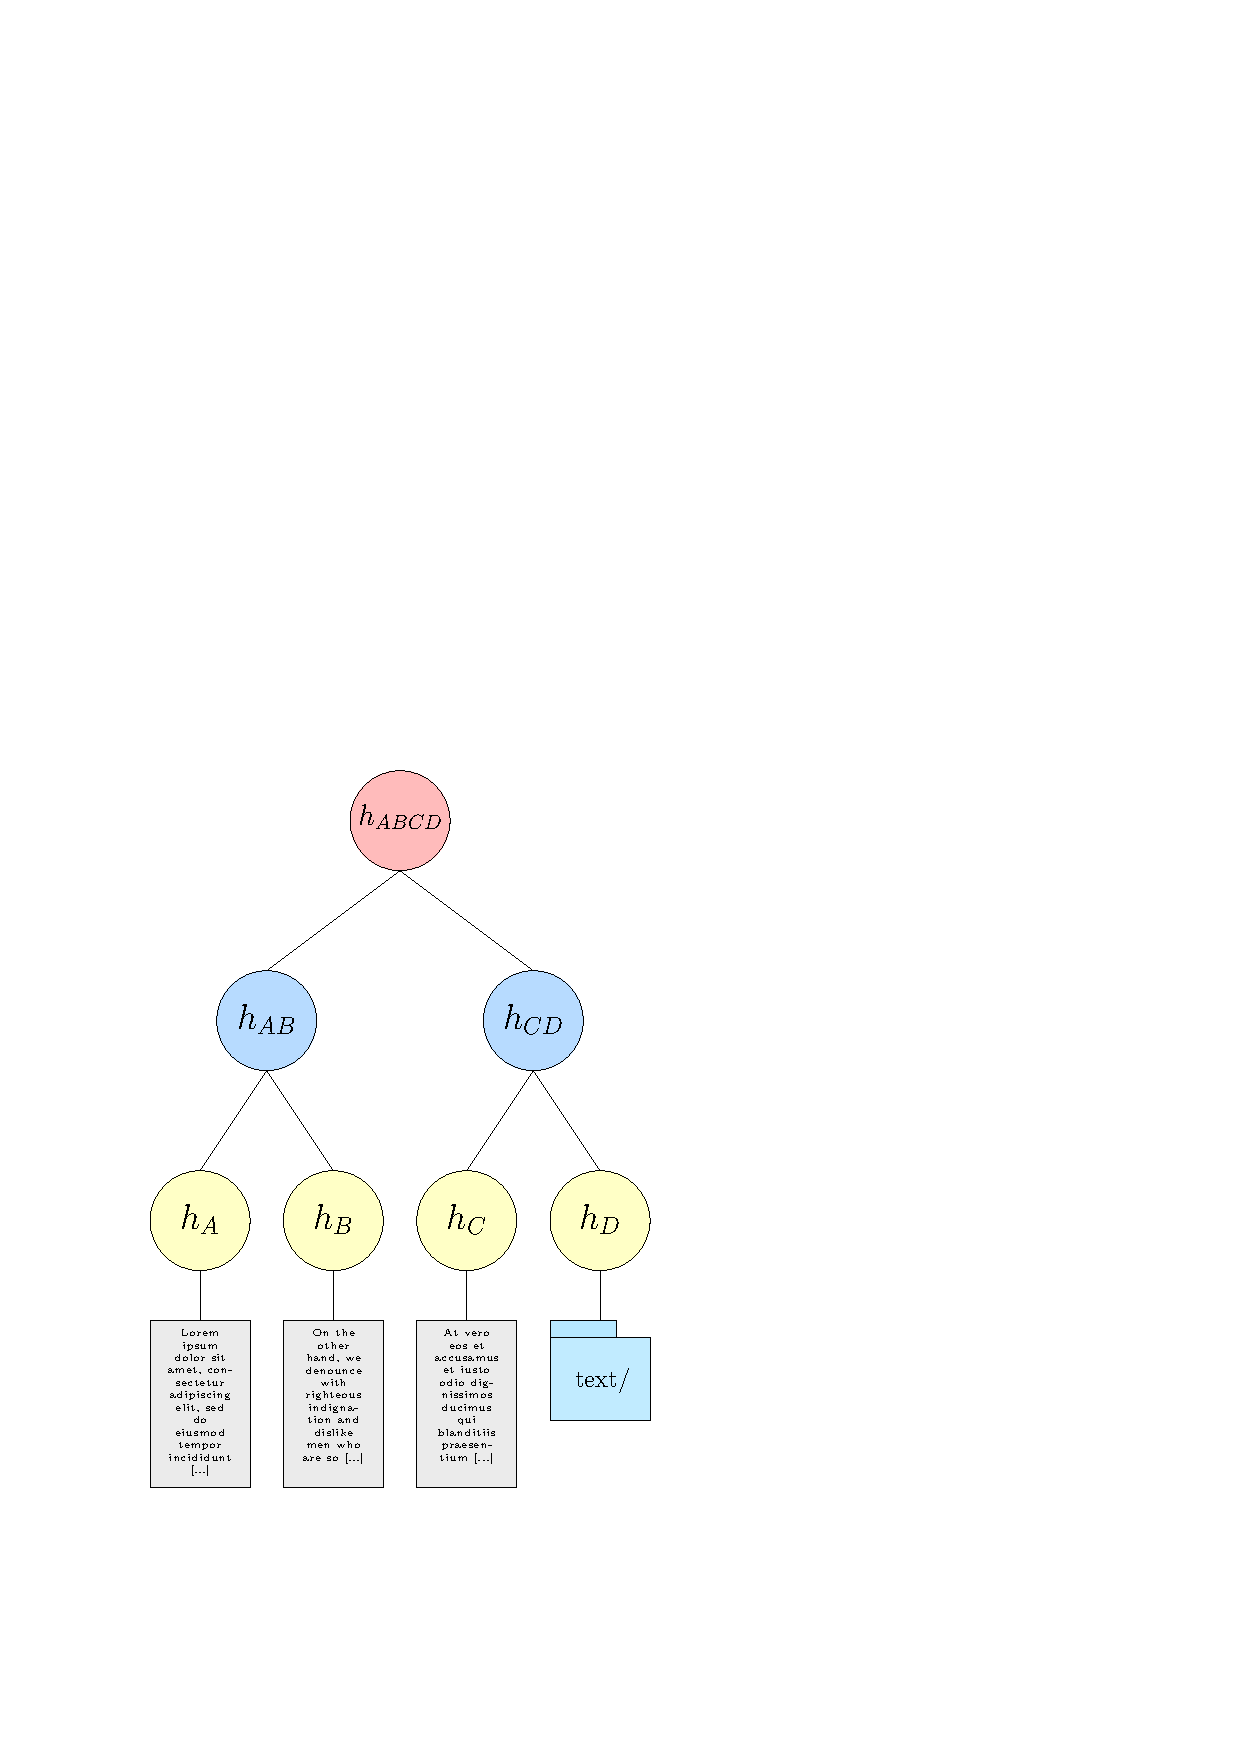
\includegraphics[width=0.4\textwidth]{mt1}
    \end{center}
    \vspace{-20pt}
\end{wrapfigure}
I Merkle Tree, nello specifico quelli binari, sono essenzialmente alberi binari
in cui ogni foglia corrisponde all’hash di uno dei nostri elementi, risalendo verso la radice ogni
nodo interno calcolerà il proprio hash concatenando gli hash dei nodi figli, infine si avrà
una radice (\textbf{Merkle Root} o MR) il cui hash è univoco a quella lista di elementi che l’albero
ha come foglie, in quella sequenza.
Inoltre, utilizzando degli hash generati con una funzione crittografica “forte”, si ha
un’assenza di collisioni tra le Merkle Root.
Perciò sappiamo che, per una determinata sequenza di documenti i cui hash sono le foglie dell'albero, anche solo una
piccola modfica ad un file causerebbe un cambiamento significativo, se non totale, della MR.

Possiamo quindi capire che c’è stato un cambiamento, tuttavia per capire anche
quale dei documenti è stato cambiato bisogna ricorrere al concetto di \textbf{Merkle Proof}.
Per effettuare una verifica tramite Merkle Proof sono tre gli elementi necessari:
\begin{enumerate}
    \item L’elemento (foglia) che vogliamo verificare
    \item La Merkle Root
    \item La Merkle Proof, ovvero la lista degli hash dei fratelli lungo il cammino dall’elemento alla matrice
\end{enumerate}
Andando a svolgere questa verifica su ogni documento riusceremo ad individuare i file modificati come
quelli per cui non è possibile ricostruire il cammino verso la radice lasciandola inalterata.

\section{JSON}
\label{sub:json}
Il JavaScript Object Notation (\textbf{JSON})~\cite{json} è un semplice formato per lo scambio di dati,
facile da interpretare e capire sia per i vari linguaggi di programmazione che per gli esseri umani.
Esso, con le librerie apposite per ogni linguaggio, permette un semplice e rapido scambio
di dati tra più applicativi e fornisce metodologie per la conversione di oggetti e collezioni
di dati strutturati in stringhe da salvare in file e viceversa, un’alternativa ragionevole ai database
per applicazioni che cercano di sviluppare architetture distribuite.
Osserviamo e analizziamo un esempio di oggetto JSON:
\begin{lstlisting}[language=json,firstnumber=1]
{ "nome": "Mario",
  "cognome": "Rossi",
  "eta": 27,
  "indirizzo": {
    "indirizzoStradale": "Via Fasulla 123",
    "citta": "Perugia"
  },
  "numeriTelefono": [
    {
      "tipo": "casa",
      "numero": "212 555-1234"
    },
    {
      "tipo": "ufficio",
      "numero": "646 555-4567"
    } ],
  "figli": [],
  "coniuge": null }
\end{lstlisting}
Possiamo osservare come ogni attributo e il suo valore vengano rappresentati come
\[``key" = value \]
dove il valore è circondato da due virgolette in caso sia una stringa (\textsf{riga 1})
o da nulla in caso sia un tipo primitivo (\textsf{riga 3}).
Un valore può inoltre essere anche un altro oggetto (\textsf{righe 4-7}), in questo caso
vediamo come sia incluso tra parentesi graffe e segua poi al suo interno la sintassi che
abbiamo appena osservato, o un array di valori semplici o oggetti (quest'ultimo alle \textsf{righe 8-16})
andando ad inserire i valori tra parentesi quadre.
È possibile anche rappresentare array vuoti (\textsf{riga 17}) con delle parentesi quadre senza
contenuto e valori nulli (\textsf{riga 18}) con la parola chiave \textsf{null}.
I valori vengono separati tra loro con una semplice virgola.

\part{Il Problema e L'Obiettivo}


La concretizzazione della soluzione al problema esposto è l’applicativo \textbf{PineSU}. \\
PineSU si presenta come un software leggero scritto in Javascript e che sfrutta il runtime Node.js.
Il software va a considerare gli insiemi di file come delle entità chiamate \\
\textbf{Storage Unit} (SU) con cui va ad avvolgere logicamente una repository Git. \\
Queste SU sono le singole unità su cui si andranno ad effettuare le singole
operazioni eccetto la registrazione su blockchain che si svolgerà collettivamente con l’ausilio di accumulatori crittografici. 

Vedremo come il ciclo di vita di una SU sia scandito dai \textbf{Blockchain Synchronization Point} (BSP),
ovvero gli eventi che si generano quando si decide di andare a registrare lo stato e la presenza di una SU su blockchain inserendola,
tramite gruppi di suoi simili chiamati \textbf{Storage Group} (SG), nella grande struttura chiamata \textbf{Merkle Calendar} (MC).
Infine, la root di questo MC sarà salvata nella Blockchain, da qui in poi sarà possibile, in qualsiasi momento, ricostruire un MC in quel preciso istante in cui un nuovo BSP è stato creato e verificare se la sua root è presente.

\section{Workflow}
\label{sec:work}

PineSU segue una filosofia di workflow che ricalca quella di Git,
infatti tramite l'applicativo si può operare su singole Storage Unit, ognuna con uno stato potenzialmente
diverso dall'altra. Ciò fa si che il workflow sia molto legato al ciclo di vita di una singola SU, la quale
a seconda del suo stato permetterà di fare alcune operazioni anziché altre.

Possiamo vederne una rappresentazione in Fig.~\ref{fi:workflow}, si parte da una directory del nostro file
system e, tramite PineSU, la si trasforma in una Storage Unit (\emph{Create new Storage Unit}) calcolandone
anche gli hash in modo da rendere già possibili registrazioni e verifiche.
Dopo questa operazione potrebbero accadere i tre eventi che seguono: 
\begin{enumerate}
    \item Il contenuto della Storage Unit potrebbe venire modificato,
    a questo punto è necessario, se si vogliono registrare anche i nuovi cambiamenti,
    andare ad effettuare un ricalcolo (\emph{Update SU}), dopo di ciò
    si torna alla possibilità dei tre eventi;
    \item Potremmo scegliere di chiudere la nostra Storage Unit (\emph{Close Storage Unit}),
    una SU è aperta (\textbf{Open}) se modificabile e ricalcolabile liberamente,
    chiusa (\textbf{Closed}) se la modifica, il ricalcolo e un’eventuale chiusura
    successiva non possono essere eseguiti, dopo la chiusura potranno essere eseguite
    in pratica le stesse operazioni eccetto, ovviamente, quella del ricalcolo;
    \item Potremmo scegliere di sincronizzare la SU nella blockchain (\emph{Synchronize with blockchain}),
    questo avviene in realtà tramite due fasi che vedremo in seguito, tuttavia
    questa scelta ci permette in seguito di eseguire qualsiasi operazione lo stesso,
    eccetto il ricalcolo nell'eventualità che questa SU sia stata chiusa precedentemente.
\end{enumerate}

Una volta che una SU è stata registrata nella blockchain o chiusa si aprono altre
due possibili azioni da poter compiere: la verifica d'integrità (\emph{Integrity verification}),
sia offline che online, l'esportazione di sottoinsiemi di file dalla SU (\emph{Export verifiable (sub)bundle}),
tutti muniti con i dati necessari per effettuare verifiche d'integrità da parte di terzi
anche senza disporre dell'intera SU.

\begin{figure}[H]
    \centering
    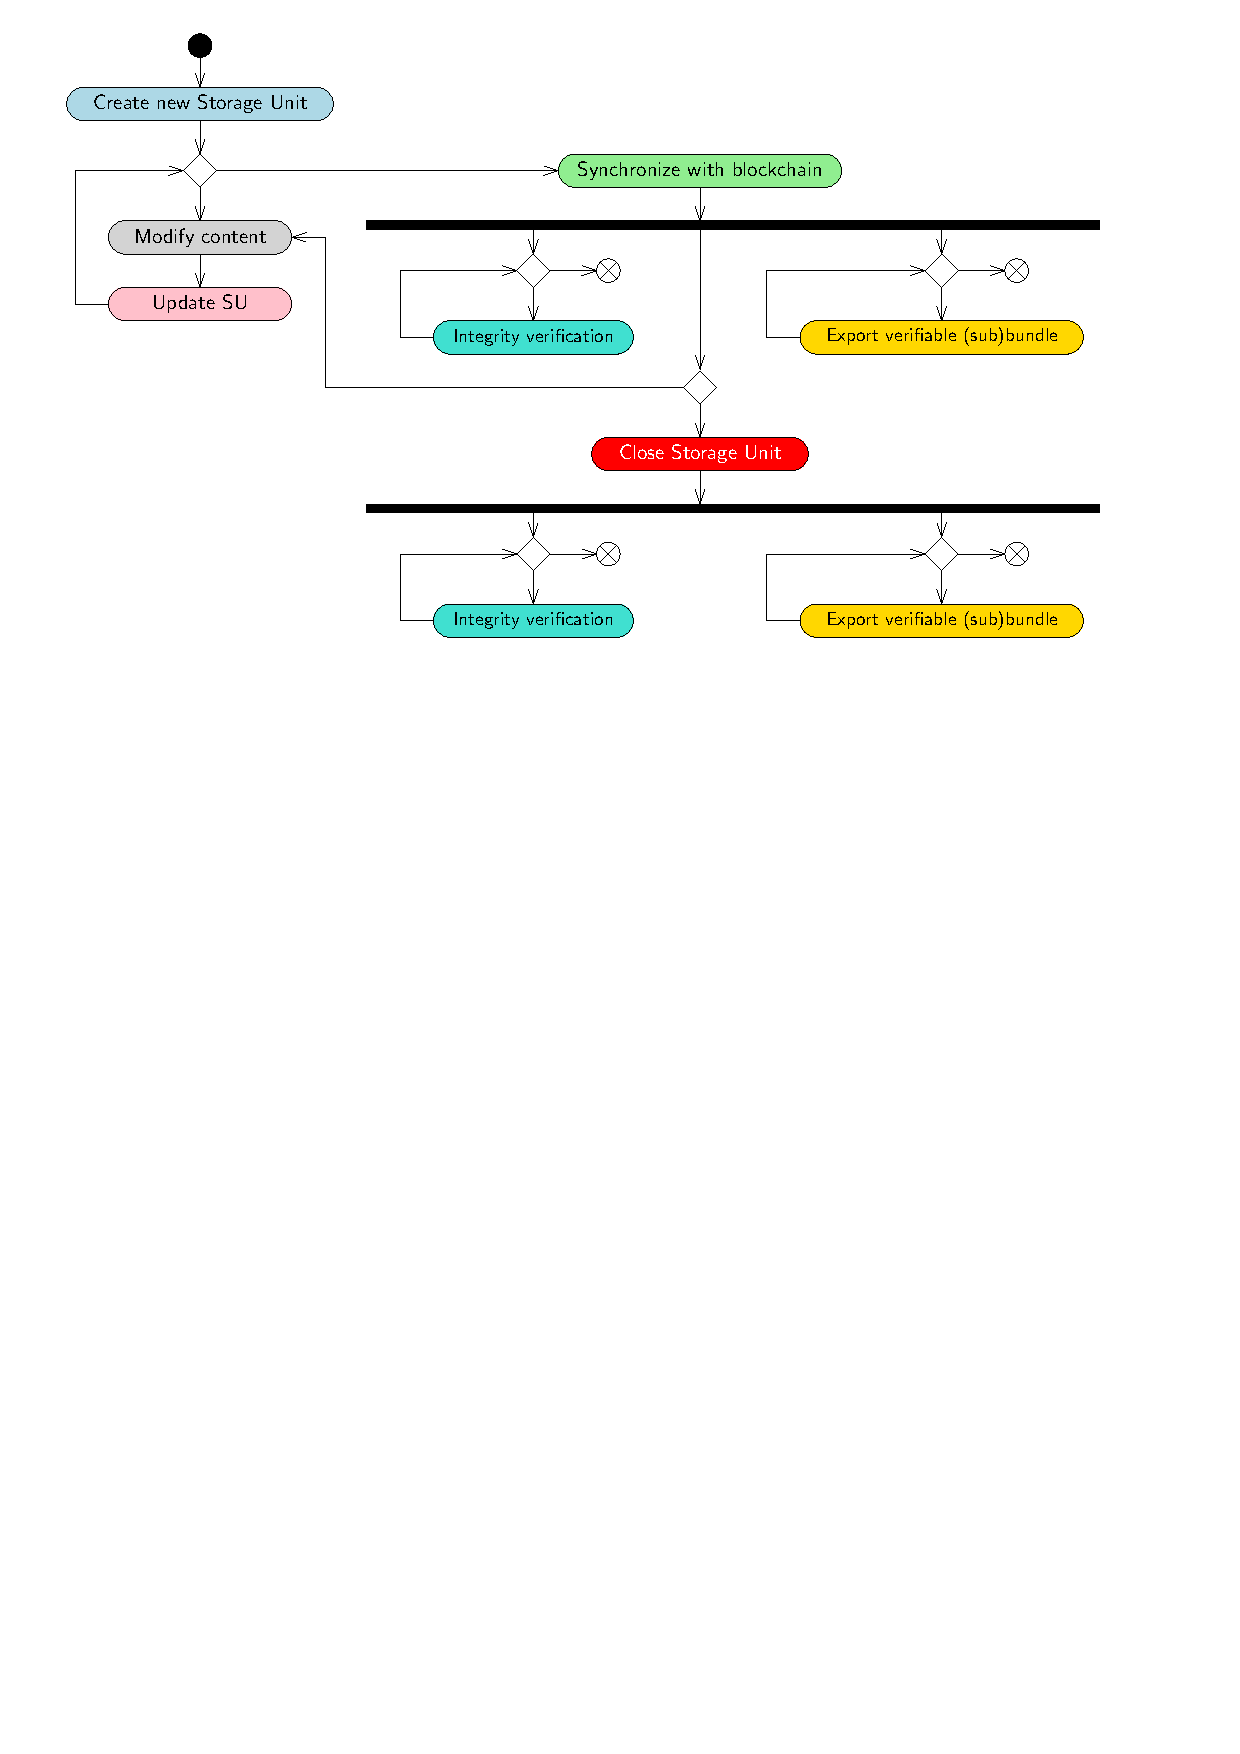
\includegraphics[width=0.98\textwidth]{Figures/activityDiag}
    \caption{\small{
    Workflow dell'applicativo sotto forma di Activity Diagram.
    } % end small
    } % end caption
    \label{fi:workflow}
\end{figure}

\newpage

Possiamo osservare il workflow appena descritto anche in Fig.~\ref{fi:stateDiag}, dove il diagramma degli
stati di una singola Storage Unit riflette le operazioni appena descritte.
Appena creata possiamo infatti riferirsci ad essa come una Storage Unit \textbf{Updated Unsynchronized Open]}
Qua da chiedere al prof. perché ne va aggiunta una: se la chiudi non è più sincronizzata per forza. 

\begin{figure}[H]
    \centering
    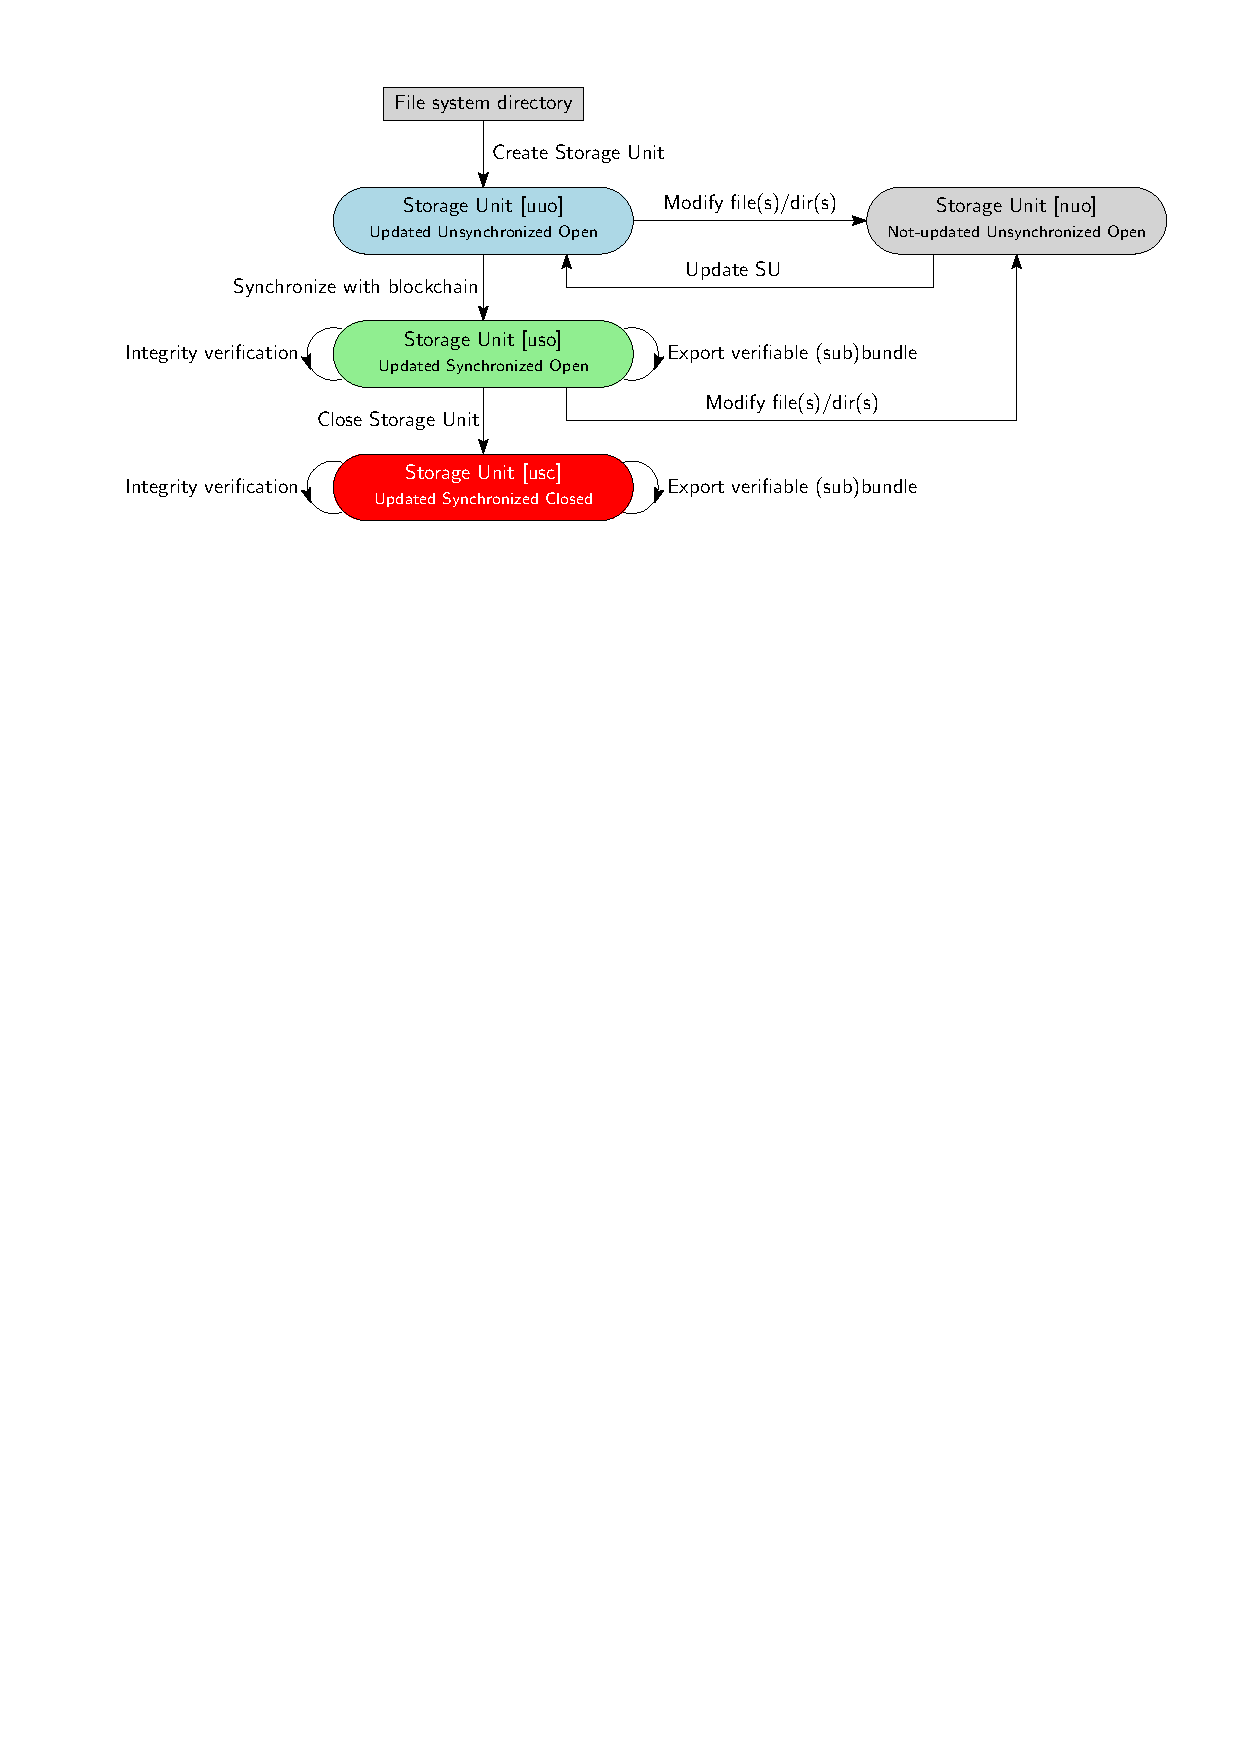
\includegraphics[width=0.98\textwidth]{Figures/stateDiag}
    \caption{\small{
    Ciclo di vita di una Storage Unit sotto forma di State Diagram.
    } % end small
    } % end caption
    \label{fi:stateDiag}
\end{figure}

\section {Architettura}
\indent
Il sistema va ad interfacciarsi con il client Git e con l’API web3.js per la comunicazione
con la blockchain Ethereum, possiamo descrivere la sua architettura come in Fig.~\ref{fi:arch}, dove troviamo i componenti principali:
\begin{itemize}
    \item \emph{PineSU \textbf{CLI} (Command Line Interface)}. L'interazione con PineSU da parte degli utenti avviene attraverso un emulatore di terminale di una macchina avente NodeJS installato\footnote{L'interfaccia si basa sul modulo npm Inquirer.js \url{https://github.com/SBoudrias/Inquirer.js}.}, analogamente a come avviene con Git, tuttavia con un'interazione più guidata. Oltre al permettere l'uso delle normali funzioni di PineSU, questo modulo permette anche l'inserimento di un qualsiasi comando di Git in modo da rendere l'utilizzo diretto di quest'ultimo non necessario durante una tipica sessione di lavoro.
    \item \emph{PineSU \textbf{BEL} (Back End Logic)}. Questo componente è il nucleo di PineSU. Gestisce tutte le SU e controlla la comunicazione con la blockchain e il client Git locale.
    Il client Git viene utilizzato inoltre per interagire indirettamente con i server Git remoti.
    Il modulo BEL, inoltre, si occupa dei due Storge Group, Open (OSG) e Closed (CSG), e
    mantiene il Merkle Tree dinamico chiamato Merkle Calendar che permette di recuperare efficientemente
    l'hash registrato in blockchain per un qualsiasi BSP. La gestione del salvataggio remoto del Merkle Calendar avviene tramite una repository Git scelta dall'utente.
    \item \emph{PineSU \textbf{EC} (Ethereum Connector)} Si interfaccia con il modulo \emph{web3.js}\footnote{\url{https://github.com/ChainSafe/web3.js}.}. 
    \item \emph{PineSU \textbf{GC} (Git Connector)} Si interfaccia con il modulo \emph{simple-git}\footnote{\url{https://github.com/steveukx/git-js}.}. 
    \item \emph{PineSU \textbf{SM} (Smart Contract)} Questo modulo entra in gioco solamente nel caso di una registrazione “forte” di una Storage Unit nella blockchain, in una fruizione standard dell’applicativo non entrerà probabilmente in azione.
\end{itemize}

\begin{figure}[H]
    \centering
    \includegraphics[width=0.98\textwidth]{Figures/PineSU-architecture}
    \caption{\small{
    Rappresentazione dell'architettura ad alto livello di PineSU. 
    Le frecce nere sono messaggi scatenati dalle entità sorgente corrispondenti
    mentre le frecce grigie sono risposte passive dell'entità interrogata.
    } % end small
    } % end caption
    \label{fi:arch}
\end{figure}

\section{Moduli in dettaglio}
\subsection{PineSU CLI}

Il modulo si occupa di creare l’effettiva interfaccia utente con cui è possibile interagire,
le domande vengono create dal modulo apposito “inquirer”, dove sono definite
insieme alle risposte possibili e ai controlli di consistenza delle risposte date dall’utente.

Dopo un setup una tantum in cui all’utente vengono chieste informazioni come gli indirizzi dei
suoi due wallet, a seconda delle scelte dall’utente, la prima di cui sarà quella dell’effettiva
operazione da eseguire (Fig.~\ref{fi:menu}), il modulo va a delineare il workflow preciso che descrive il ciclo vitale
di una SU, il tutto richiamando all’occorrenza le librerie del modulo \emph{PineSU BEL}. 

\begin{figure}[H]
    \centering
    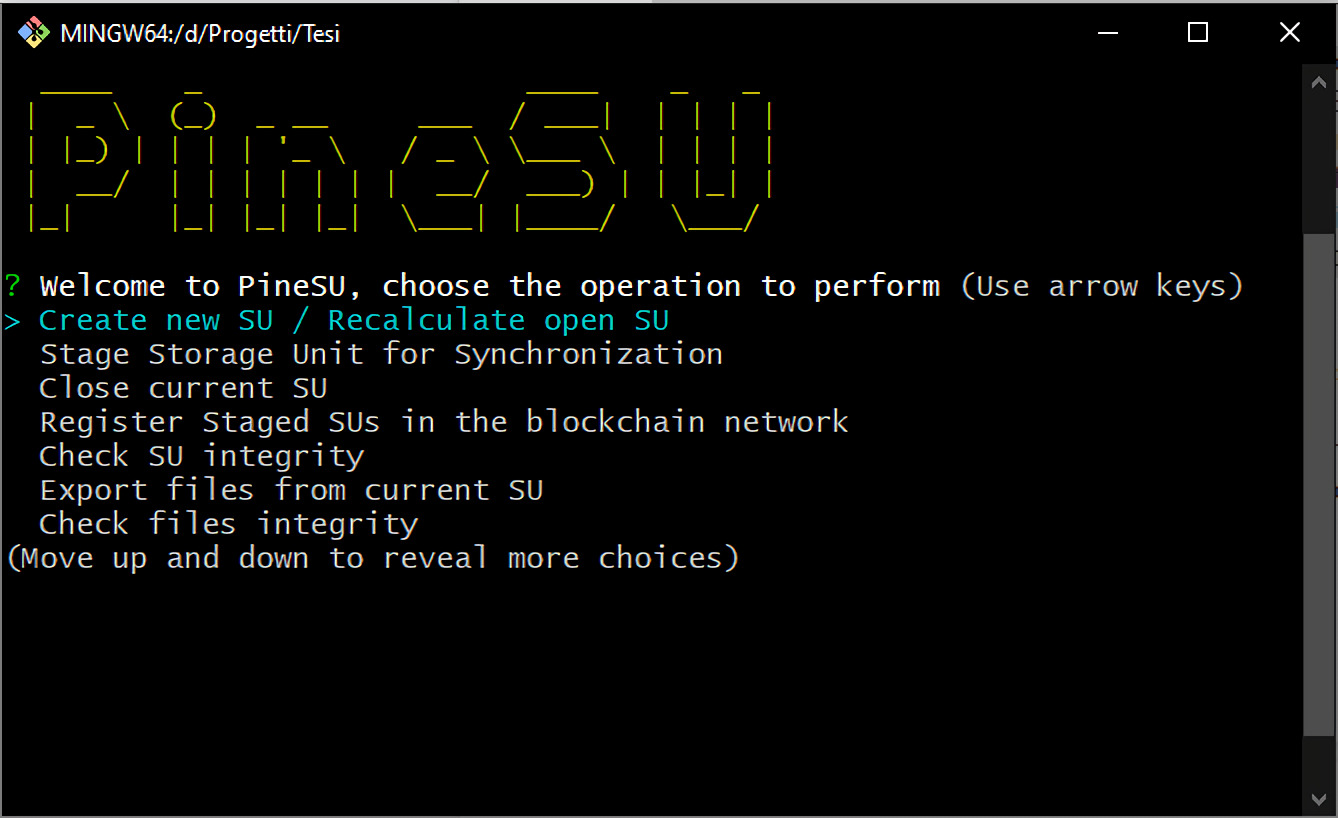
\includegraphics[width=0.98\textwidth]{Figures/menu}
    \caption{\small{
    Menù principale dell'applicativo con la scelta dell'operazione da effettuare.
    } % end small
    } % end caption
    \label{fi:menu}
\end{figure}

\subsection{PineSU BEL}

Questo modulo è il nucleo centrale del software, si occupa dell’effettiva comunicazione con i connettori per Git e per la blockchain, del gestire il File System andando a leggere e scrivere i file all’interno delle Storage Unit, di assegnare stringhe crittografiche ai singoli file e di creare e gestire le strutture di accumulazione crittografica.

Per la prima delle operazioni sopra citate troviamo due librerie, rispettivamente \textbf{GitLogic} e \textbf{EthLogic}, le quali si occupano essenzialmente di creare oggetti delle rispettive classi di connettori, reperire tramite altre librerie le informazioni necessarie, chiamare le funzioni dei connettori con gli input dovuti e gestire gli output in maniera coerente con ciò che necessita \emph{PineSU CLI}.

Andiamo ora a vedere le due classi che si occupano di creare e gestire le strutture di memorizzazione che il programma utilizza: \textbf{Files} e \textbf{TreeList}.
Files si occupa della lettura di file JSON, la lettura dei file di cui andrà letta la stringa hash corrispondente e della scrittura dei file JSON. Questi file JSON corrispondono ai descrittori delle SU (riguardanti la creazione e la registrazione su blockchain), alle informazioni sull’utente utilizzatore e alle strutture degli accumulatori crittografici.
\newpage
TreeList si occupa del reperimento delle stringhe di hash e del calcolo dei Merkle Tree binari.
Essi sono fondamentali per varie operazioni che vanno dal calcolo degli hash delle directory al quello della creazione dei tre accumulatori crittografici che andremo ora a descrivere.
\\ Il primo è il semplice SU Merkle Tree, necessario per il calcolo dell’hash corrispondente alla Storage Unit, che altro non è che un Merkle Tree binario in cui ogni foglia corrisponde a un file o una directory contenuta nella SU. Questo MT verrà utilizzato anche nella fase di esportazione per generare le proof dei file esportati che serviranno per un eventuale controllo d’integrità singolo.
\\ Il secondo è lo Storage Group, di cui ne esistono due, un \textbf{Open} (OSG) e un \textbf{Closed} (CSG). Si tratta essenzialmente di due MT binari in cui ogni foglia corrisponde all’hash di una Storage Unit \textbf{Staged}, la differenza tra i due alberi è nel loro contenuto, uno contiene le SU Open, l’altro le SU Closed, differenza già discussa nella \autoref{sec:work}. Le root di questi alberi verranno poi salvate all’interno della prossima struttura come foglie.
\\ Il terzo e il più importante è il \textbf{Merkle Calendar}, formato da due sottoalberi in cui vengono accolte come foglie rispettivamente le istanze di OSG e di CSG. Le radici di questi due sottoalberi hanno come figli dei nodi corrispondenti agli anni, i quali a loro volta hanno come figli dei nodi corrispondenti ai mesi, i figli dei mesi saranno infine le foglie corrispondenti a ciò che chiamiamo \textbf{Blockchain Synchronization Point} (BSP) in quanto nodi contenenti un timestamp e la root dello SG corrispondente.
\\
Possiamo vedere, anche grazie a Fig.~\ref{fi:umlMC}, come questa struttura sia implementata tramite tre classi:

\begin{itemize}
    \item \textbf{MerkleCalendar}: contiene i riferimenti alle due radici dei sottoalberi e mette a disposizione varie funzioni per la ricerca di hash e reperimento di determinati valori della root in un certo BSP.
    \item \textbf{InternalCalendar}: corrisponde a un nodo interno dell’albero, quando si aggiungono figli si può scegliere di effettuare il ricalcolo del loro hash in modo da non doverlo calcolare successivamente (semplifica l’operazione di reperimento dell’hash di un certo BSP).
    \item \textbf{LeafCalendar}: corrisponde a una foglia dell’albero.
\end{itemize}


\begin{figure}[H]
    \centering
    \resizebox{0.9\textwidth}{!}{
        \begin{tikzpicture}
            \begin{class}[text width=14cm]{MerkleCalendar}{0,0}
                \attribute{}
                \operation{+ addRegistration(name: string, hash: string, date: Date, closed: boolean): void}
                \operation{+ getBSPRoot(hash: string, oHash: string, cHash: string): string}
                \operation{+ getTrees(): [Array, Array]}
            \end{class}
            \begin{class}[text width=9.5cm]{InternalCalendar}{4,-4.5}
                \attribute{- name : string}
                \attribute{- category : int}
                \attribute{- parent : InternalCalendar}
                \attribute{- category : int}
                \attribute{- hash : string}
                \operation{constructor(name: string, category: int, parent: Object)}
                \operation{+ addChild(node: Object) : void}
                \operation{+ calculateHash() : void}
                \operation{+ getChildByName(name: string) : Object}
                \operation{+ findNode(hash: string) : Object}
            \end{class}
            \begin{class}[text width=15cm]{LeafCalendar}{2,-12.5}
                \attribute{- name : string}
                \attribute{- day : int}
                \attribute{- hour : InternalCalendar}
                \attribute{- minute : int}
                \attribute{- hash : string}
                \operation{constructor(name: string, day: int, hour: int, minute: int, hash: string, parent: Object)}
            \end{class}
            \composition{MerkleCalendar}{open, closed}{2}{InternalCalendar};
            %\aggregation{InternalCalendar}{children}{0..*}{LeafCalendar};
            %\aggregation{LeafCalendar}{parent}{0..1}{InternalCalendar};
            \aggregation{[xshift=2cm] InternalCalendar.south}{0..*}{children}{[xshift=2cm] LeafCalendar.north};
            \composition{[xshift=-2cm] LeafCalendar.north}{1}{parent}{[xshift=-2cm] InternalCalendar.south};
            %\aggregation{[xshift=-2cm] A}{second}{1}{[xshift=-2cm] B.north};
            \selfAssociation{InternalCalendar}{parent}{0,1};
        \end{tikzpicture}
    }
    \caption{Rappresentazione UML delle classi descritte} \label{fi:umlMC}
\end{figure}

\newpage

\subsection{Excursus sul Merkle Calendar}

In Fig.~\ref{fi:mcIPE} possiamo osservare un possibile Markle Calendar.
Nell'esempio è stato esplorato il mese di Febbraio 2021 e lì troviamo tre BSP:
esse corrispondono a tre registrazioni della root dell'intero MC su blockchain, ovviamente
sempre diversa dato che l'hash root si calcola con gli hash delle sue foglie.

\begin{figure}[H]
    \centering
    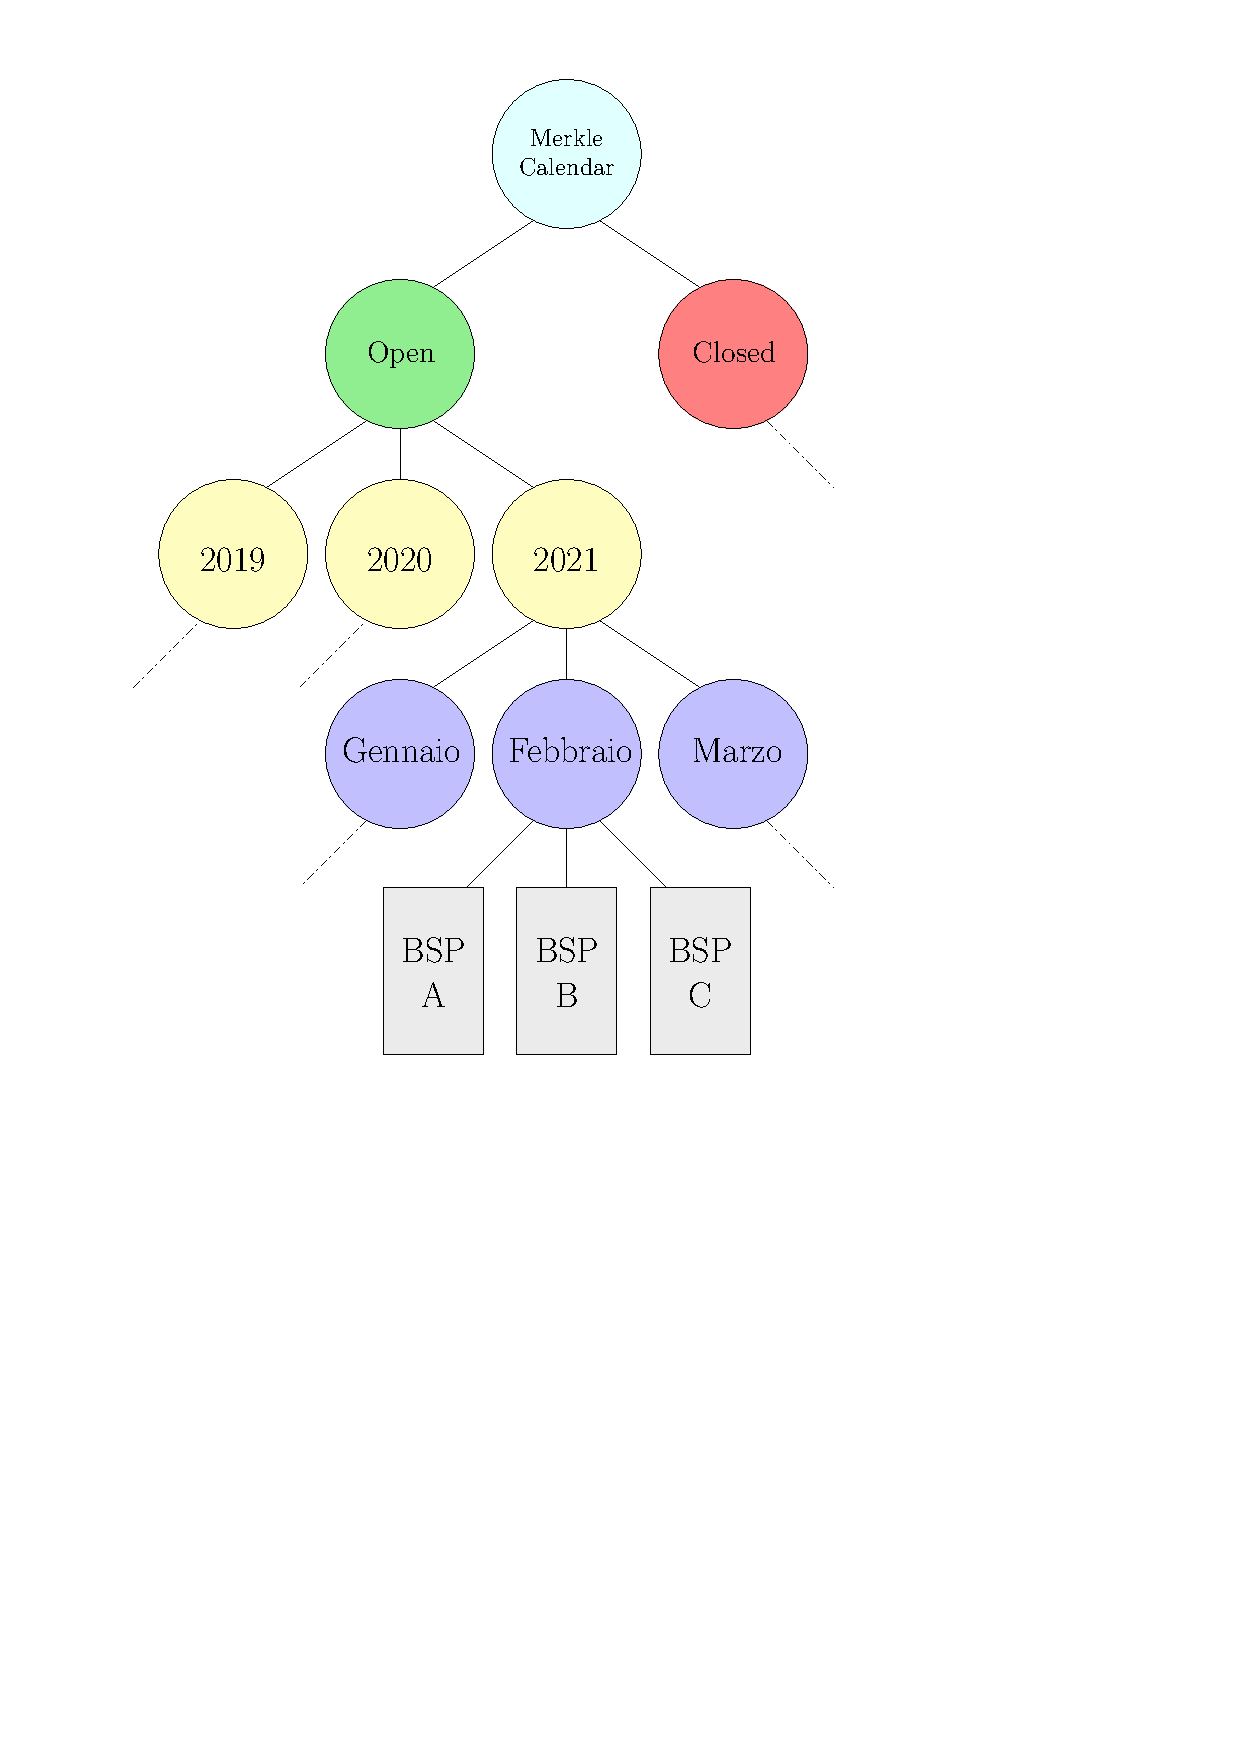
\includegraphics[width=0.5\textwidth]{Figures/mc1}
    \caption{\small{
    Rappresentazione grafica di un Merkle Calendar.
    } % end small
    } % end caption
    \label{fi:mcIPE}
\end{figure}

Ogni volta che un nuovo BSP viene inserito per la prima volta si avvia la procedura di
ricalcolo dell'hash di ognuno dei suoi antenati in modo da non dover effettuare il calcolo
dell'hash di gran parte dell'albero nella fase di reperimento.

Nel momento in cui ognuna di queste tre BSP è stata inserita nell'albero essa era la foglia più
giovane, ergo se volessimo calcolare la root del MC in una data BSP ci basterebbe non
considerare tutto ciò che è stato inserito successivamente, andando ad escludere una
partizione di estrema destra dal sottoalbero radicato in Open (in questo caso).

Ipotizziamo di voler recuperare la MC root nel momento in cui è stata inserita BSP B:
\begin{enumerate}
    \item Calcoliamo l'hash di Febbraio tramite l'hash di BSP a e di BSP B;
    \item Calcoliamo l'hash del 2021 tramite l'hash di Gennaio e il “nuovo” hash di Febbraio;
    \item Calcoliamo l'hash di Open tramite gli hash del 2019, del 2020 e il “nuovo” hash del 2021;
    \item Calcoliamo la root del MC tramite l'hash di Closed e il “nuovo” hash di Open, l'hash di Closed nell'istante dell'inserimento di BSP B viene salvato in un descrittore JSON presente in ogni SU registrata con BSP B.
\end{enumerate}
Il calcolo di hash tramite altri hash è effettuato tramite dei piccoli Merkle Tree binari “usa e getta”, alla stessa maniera di come calcoliamo l'hash root di uno Storage Group (che andrà a finire nei BSP foglia dei MC).

\subsection{PineSU EC}

Come visualizzabile in Fig.~\ref{fi:umlEC} il connettore per la blockchain, in questo caso specifico quello della rete Ethereum, è composto da una semplice classe che, con i suoi attributi che corrispondono ad un oggetto del modulo web3.js, i due indirizzi dei wallet e la chiave privata del primo, svolge le operazioni di effettuare una transazione e verificarne una precedente.

\begin{figure}[H]
    \centering
    \resizebox{0.65\textwidth}{!}{
        \begin{tikzpicture}
            \begin{class}[text width=10.5cm]{EthConnector}{0,0}
                \attribute{- web3 : Web3}
                \attribute{- w1 : string}
                \attribute{- w2 : string}
                \attribute{- k : string}
                \operation{constructor(host: string, w1 : string, w2 : string, k : string)}
                \operation{+ addChild(node: Object) : void}
                \operation{+ calculateHash() : void}
                \operation{+ getChildByName(name: string) : Object}
                \operation{+ findNode(hash: string) : Object}
            \end{class}
        \end{tikzpicture}
    }
    \caption{Rappresentazione UML di EthConnector}
    \label{fi:umlEC}
\end{figure}


\subsection{PineSU GC}

Il connettore per Git, la cui rappresentazione UML è visualizzabile in Fig.~\ref{fi:umlGC},
è una semplice classe che lavora con un attributo della classe proveniente
dal modulo simple-git, essa prende in input una directory su cui lavorare
ed è poi in grado, in base alle chiamate delle funzioni del connettore, di operare su di
essa tramite il client Git installato sulla macchina.

\begin{figure}[H]
    \centering
    \resizebox{0.52\textwidth}{!}{
        \begin{tikzpicture}
            \begin{class}[text width=8cm]{GitConnector}{0,0}
                \attribute{- git : SimpleGit}
                \operation{constructor(dir: string)}
                \operation{+ init() : void}
                \operation{+ add(arg: string) : void}
                \operation{+ commit(msg: string, enmsg: boolean) : void}
                \operation{+ getRepoFiles() : Array}
                \operation{+ push() : void}
                \operation{+ pull() : void}
                \operation{+ reset() : void}
                \operation{+ hasRemote() : Array}
                \operation{+ custom(commands: Array) : string}
            \end{class}
        \end{tikzpicture}
    }
    \caption{Rappresentazione UML di GitConnector}
    \label{fi:umlGC}
\end{figure}

\subsection{PineSU SM}
\label{sub:sm}
Lo Smart Comtract (\autoref{sub:smp}) di PineSU è necessario
per poter effettuare registrazioni “forti”, ovvero andare a salvare su blockchain
che una determinata SU è stata chiusa in modo da evitare che delle eventuali manomissioni
cerchino di chiuderla nuovamente (ricordiamo che una SU chiusa implica un'impossibilità di modifica e ricalcolo).
Questo modulo è presente solamente in caso si vadano ad utilizzare blockchain di criptovalute che
supportano la presenza di Smart Contract, nel nostro caso, con Ethereum, siamo a posto.
Questo modulo non è tutt'ora implementato ed è destinato a sviluppi futuri \autoref{}.

\section{Funzionalità}

L’elenco delle funzionalità è il seguente.

\begin{enumerate}
    \item Creazione di una Storage Unit o Ricalcolo di una Storage Unit pre-esistente
    \item Staging di una Storage Unit nello Storage Group
    \item Registrazione dello Storage Group nella Blockchain
    \item Chiusura di una Storage Unit
    \item Esportazione di sottoinsiemi di file da una SU
    \item Controllo di integrità di singoli file esportati da altre SU
    \item Controllo di integrità su una SU
\end{enumerate}

Alle operazioni che implicano modifiche alla struttura o allo stato della SU seguirà sempre un Git commit.
Andremo ora ad analizzarle una per volta.

\subsection{Creazione di una Storage Unit o Ricalcolo di una Storage Unit pre-esistente}
La creazione di una Storage Unit è in realtà un'operazione che comprende sia la trasformazione in una Git Repository della directory, sia il calcolo degli hash che serviranno poi per registrare la nostra SU nella blockchain. Le informazioni della nostra SU sono conservate nel file descrittore \textbf{.pinesu.json} nella root della directory, la presenza di questo file indica al programma che la directory è già una SU. Anche nel caso in cui .pinesu.json sia già presente nella directory questa operazione può essere eseguita e provvederà al ricalcolo degli hash e la creazione di un nuovo descrittore, questo ovviamente solo se la SU è aperta.
Dei file possono essere esclusi dalla Storage Unit con l’ausilio di un semplice file \emph{.gitignore}, la cui creazione viene anch’essa gestita, in maniera opzionale, dal software.

\subsection{Staging di una Storage Unit nello Storage Group}
Lo hash principale della Storage Unit viene inserito in uno dei due Storage Group (a seconda che sia aperta o chiusa), questa operazione è stata nominata \emph{staging} in quanto è concettualmente simile all’operazione omonima di Git se consideriamo la registrazione nella Blockchain analoga ad un \emph{commit}.

\subsection{Registrazione dello Storage Group nella Blockchain}
Le root dei due Storage Group vengono inserite nel Merkle Calendar, si effettua una transazione tra due wallet contenente la nuova root del Merkle Calendar.
Gli SG vengono poi svuotati e le proof per essere dinamicamente ricostruiti vengono salvate, insieme alle informazioni per reperire la transazione, in un descrittore JSON nelle directory delle varie Storage Unit appena registrate.

\subsection{Chiusura di una Storage Unit}
La Storage Unit viene chiusa ma ad una condizione che varia a seconda dei casi:
\begin{itemize}
    \item \emph{Weak}: Si controllano i commit della repository per controllare che un commit di chiusura sia già avvenuto.
    \item \emph{Strong}: Si controlla la blockchain, tramite PineSU SM (\autoref{sub:sm}), per verificare che sia presente la entry corrispondente alla chiusura di quella SU.
\end{itemize}

\subsection{Esportazione di sottoinsiemi di file da una SU}
In questa fase all'utente viene data la possibilità di scegliere di esportare alcuni file dalla SU, viene creato un file \textbf{.pifiles.json} in cui si salva, per ogni file esportato, il suo percorso originale, il suo hash, l'hash della root e le \emph{proof} per calcolare la root dato l'hash del file (ciò servirà nell'operazione di verifica d'integrità). Infine i file, seguendo la struttura in cui comparivano nella SU originale, e .pifiles.json vengono compressi in un file ZIP e salvati nella cartella precedente a quella in cui si sta operando.

\subsection{Controllo di integrità di singoli file esportati da altre SU}
Viene analizzata la directory in modo da trovare dei file descrittori \textbf{.pifiles.json}, da quelli e dai file in essi elencati si fa un controllo d’integrità che va anche ad effettuare lo stesso controllo su Blockchain che si effettua nell’ultima operazione.

\subsection{Controllo di integrità su una SU}
Si legge la root dello Storage Group della SU selezionata e si cerca tale root nel Merkle Calendar, una volta trovato si è in grado di ricalcolare la root del Merkle Calendar nel momento in cui tale Storage Group è stato registrato, da qui si controlla se la transazione salvata contiene anch’essa la root del Merkle Calendar come messaggio.


\part{Il Software PineSU}

In questo capitolo andremo a testare l'applicativo mostrando cosa accade nel
file system ogni volta che PineSU esegue una funzione.
Prenderemo in esame una situazione in cui creeremo due SU, una verrà lasciata aperta,
l'altra verrà prima registrata aperta, poi chiusa e registrata nuovamente, in questo modo
riusciremo anche ad osservare i cambiamenti sull'intero Merkle Calendar.

\section{Prima inizializzazione}

Alla prima apertura di PineSU sulla macchina il processo ci andrà a chiedere
quattro valori: due indirizzi di Wallet Ethereum, la chiave privata del primo dei wallet e,
opzionalmente, la repository Git remota con cui sincronizzare il MerkleCalendar

\section{Creazione delle Storage Unit}

Partiamo definendo il contenuto delle nostre due directory, la prima,
\textbf{\textsf{sample}}, ha questa struttura:
\begin{itemize}
    \itemsep0em
    \item sample/graphCreator.js
    \item sample/first/astar.js
    \item sample/first/graph.js
    \item sample/second/priorityQueue.js
    \item sample/second/third/main.js
    \item sample/second/third/vertex.js
\end{itemize}
Dove \textsf{first} e \textsf{second} sono due subdirectory di \textsf{sample}
e \textsf{third} è una subdirectory di \textsf{second}. \\
I file contenuti sono dei file plain text salvati in formato JavaScript. \\ \\
La seconda directory, \textbf{\textsf{secondSample}}, ha questa struttura:
\begin{itemize}
    \itemsep0em
    \item \textsf{secondSample/esonero1/Immagine.png}
    \item \textsf{secondSample/esonero1/preesonero.pdf}
    \item \textsf{secondSample/esonero1/preesonero.tex}
    \item \textsf{secondSample/esonero2/preesonero2.pdf}
    \item \textsf{secondSample/esonero2/preesonero2.tex}
    \item \textsf{secondSample/esonero3/preesonero3.pdf}
    \item \textsf{secondSample/esonero3/preesonero3.tex}
    \item \textsf{secondSample/esonero3/smith-chart.png}
\end{itemize}

Dove \textsf{esonero1}, \textsf{esonero2} ed \textsf{esonero3} sono tre subdirectory di \textsf{secondSample}.
In questa directory troviamo anche la presenza di file di diversa natura. \\


Per trasformare le directory in Storage Unit posizioniamoci con il terminale all'interno di ognuna,
avviamo lo script di avvio di PineSU e selezioniamo la prima opzione (\emph{Create / Recalculate SU}),
ovviamente il procedimento andrà ripetuto due volte.
Il processo ci chiederà se inizializzare una repository Git e se escludere alcuni file,
procederà poi al calcolo dei vari hash.

\begin{figure}[H]
    \centering
    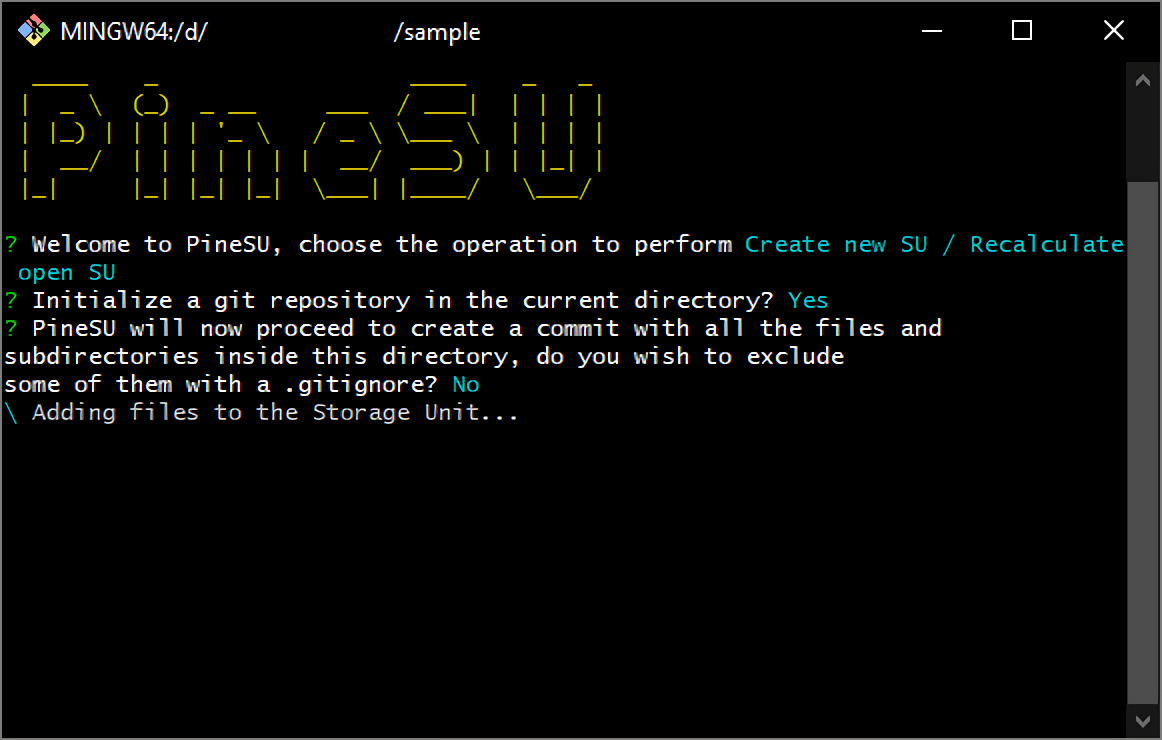
\includegraphics[width=0.9\textwidth]{Figures/calculating}
    \caption{\small{
    L'interfaccia di PineSU durante il calcolo.
    } % end small
    } % end caption
    \label{fi:calc}
\end{figure}


Una volta finito di calcolare ci verranno fatte domande sulla natura della Storage Unit come il suo nome,
la repository remota a cui si sincronizza, la sua descrizione, ecc\dots \\
Finite le domande, l'applicativo ci riporterà al menù principale.

\begin{figure}[H]
    \centering
    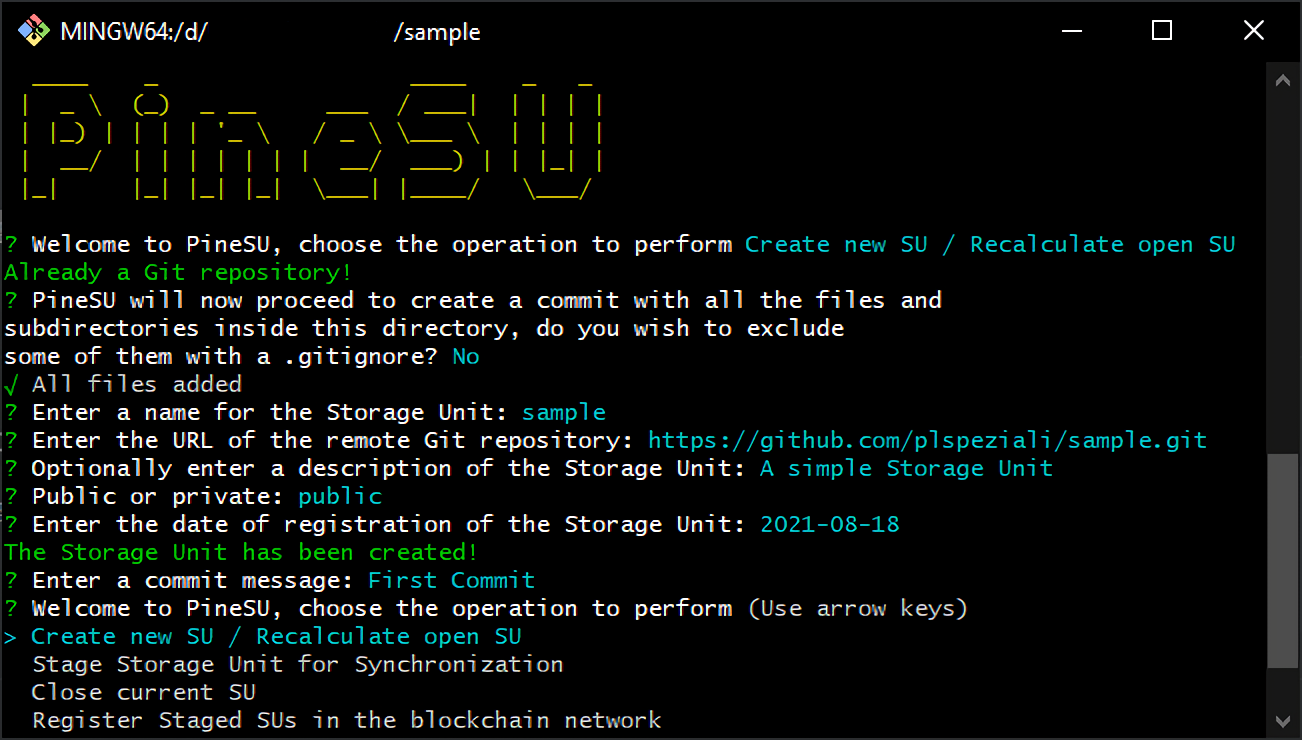
\includegraphics[width=0.9\textwidth]{Figures/doneCalculating}
    \caption{\small{
    L'interfaccia di PineSU appena terminata la fase di creazione.
    } % end small
    } % end caption
    \label{fi:dcalc}
\end{figure}

Al termine di entrambe le elaborazioni sulle due directory avremo alcune nuove aggiunte al loro interno:
una cartella .git (eventualmente, anche un file .gitignore) e un file .pinesu.json, quest'ultimo è
il descrittore JSON in cui sono salvate le informazioni che abbiamo inserito, gli hash calcolati e
lo stato di chiusura. Ecco, ad esempio, il file JSON di \textsf{sample}:

\begin{lstlisting}[language=json,firstnumber=1]
{"name": "sample",
"remote": "https://github.com/plspeziali/sample",
"description": "A simple Storage Unit",
"visibility": "public",
"date": "2021-08-18",
"owner": "0xCF23544bFC002905532bD86bF647754A84732966",
"hash": "3837ec6fe66032ba593d227ee800a079c61a5853",
"filelist": [
    "first/astar.js:e09deffb3654301a9a8d20acc5a7091cda7039b6",
    "first/graph.js:53982e4feeaf1445434864b409014706e31da1cc",
    "graphCreator.js:c3b4338c33d6ea5a30b31c16defc7661a4ae767b",
    "second/priorityQueue.js:1cb66abaaafd6a7125ab7dac1d7e0fb1860da574",
    "second/third/main.js:1b8dad338691dead8edc66e7c01b8db6d834e3d8",
    "second/third/vertex.js:aa3fa9242ceec7062c7d84764e4068711e53c4e3",
    "first:75d936d52208d14c2cd571e0c595bc29e7d0e3a0",
    "second/third:2ec86afc483f3685893831dfe04b66620be690d2",
    "second:d6e51cdbe8a84cb3ba2c9cfdc2773a96b2401a59"
],
"closed": false }
\end{lstlisting}
\newpage

\section{Staging delle Storage Unit}

A questo punto vogliamo registrare le nostre Storage Unit aperte nella blockchain, 
occorre però prima inserirle negli Storage Group
(in questo caso solo in Open Storage Group).
Per effettuare questa operazione occorre solo selezionare l'opzione apposita (\emph{Stage SU for Synchronization})
in entrambe le directory, nella nostra cartella d'installazione verrà 
aggiornato il file \textsf{merkles/storageGroup.json} con le informazioni delle nostre SU.

\begin{lstlisting}[language=json,firstnumber=1]
[ {
    "name": "sample",
    "hash": "3837ec6fe66032ba593d227ee800a079c61a5853",
    "path": "D:/sample",
    "closed": false
  },
  {
    "name": "secondSample",
    "hash": "7a61ed5e43cd436fb1f88895625a8193fdb9b3be",
    "path": "D:/secondSample",
    "closed": false
  } ]  
\end{lstlisting}
Questa è la lista delle foglie con cui calcoleremo l'effettivo Merkle Tree di OSG.

\section{Registrazione su Blockchain}
\label{sub:regbc}
Per la registrazione non è necessario posizionarsi in una delle directory delle SU
in quanto quelle da registrare sono già nello Storage Group, ci rimane solo
da selezionare l'opzione apposita (\emph{Register Staged SUs}) per eseguire
con la registrazione, a questo punto lo Storage Group verrà svuotato
e verrà popolato, almeno nel sottoalbero Open, il Merkle Calendar con una foglia
in più e, all'occorrenza, dei nodi interni extra (in caso non fossero state
registrate delle SU in questo mese e anno).

Ovviamente di conseguenza la nuova Merkle Root del Merkle Calendar verrà registrata su
blockchain Ethereum inserendola in un messaggio scambiato tra i due wallet forniti dall'utente,
ciò non è visualizzabile dall'utente a meno che non vada nelle directory delle SU registrate 
in cui potrà trovare un nuovo file \textsf{.registration.json}, esso conterrà informazioni
come la root dello Storage Group in cui è stato registrato, la proof per ricostruire tale root,
l'hash della transazione per recuperarla dalla catena e gli hash dei sottoalberi Open e Closed
del MerkleCalendar nel momento in cui è stato registrato.
\newpage
\begin{lstlisting}[language=json,firstnumber=1]
    { "path": "D:/Progetti/Tirocinio/sample",
    "root": "e67006f15ecd3fa2719d148be68d3a3242e1be8b",
    "proof": [ {
     "right": "7a61ed5e43cd436fb1f88895625a8193fdb9b3be"
    } ],
    "transactionHash": "0xc56303032[...]2dc87d2e",
    "oHash": "e67006f15ecd3fa2719d148be68d3a3242e1be8b",
    "cHash": null }  
\end{lstlisting}

\section{Verifica d'integrità di una Storage Unit}

A questo punto ci troveremo ad avere Storage Unit USO (Updated Synchronized Open), ciò
significa che ha senso sia effettura verifiche d'integrità avvalendoci della blockchain,
sia esportare sottoinsiemi di file da essa in modo che anche chi reperisce tali file sia
in grado di verificare la loro integrità e la loro registrazione su blockchain.
La verifica può essere fatta selezionando l'opzione \emph{Check SU integrity}
mentre ci si trova nella directory della SU da verificare, il successo o
l'insuccesso ci verranno comunicati su schermo.

\begin{figure}[H]
    \centering
    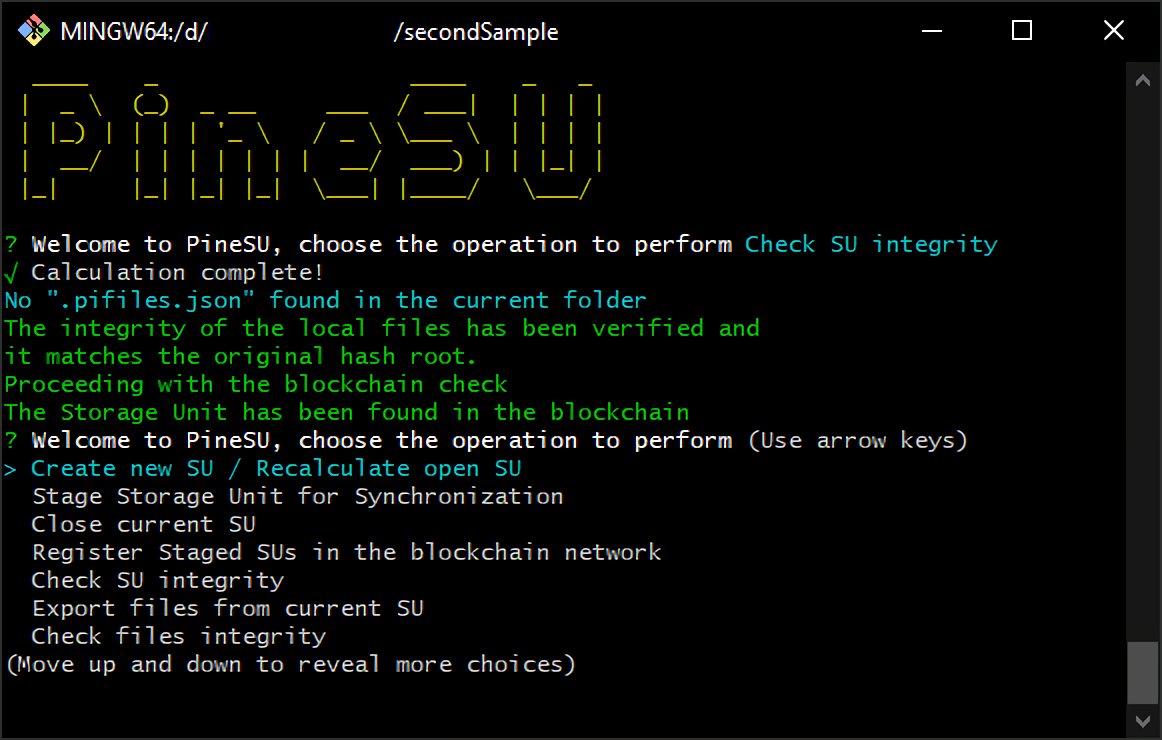
\includegraphics[width=0.9\textwidth]{Figures/verify}
    \caption{\small{
    L'interfaccia di PineSU appena terminata la fase di verifica con successo.
    } % end small
    } % end caption
    \label{fi:ver}
\end{figure}
\newpage

\section{Esportazione di file da una Storage Unit}
\label{sub:exp}
Per quanto riguarda l'esportazione di file, andremo ad eseguirla su \textsf{secondSample}.
Essa viene eseguita selezionando i file da esportare con l'apposita interfaccia
di selezione multipla
\begin{figure}[H]
    \centering
    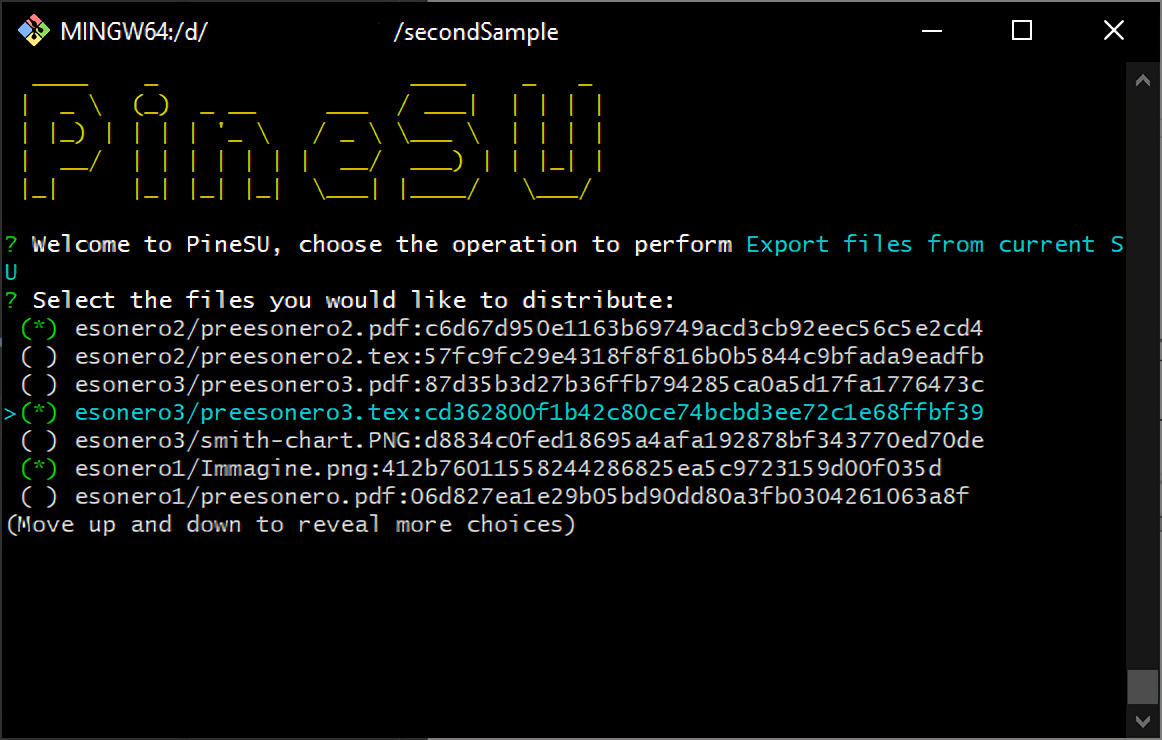
\includegraphics[width=0.9\textwidth]{Figures/export}
    \caption{\small{
    L'interfaccia di PineSU durante un'esportazione.
    } % end small
    } % end caption
    \label{fi:exp}
\end{figure}

In questo caso siamo andati a selezionare \textsf{esonero2/preesonero2.pdf},
\textsf{esonero3/preesonero3.tex} e \textsf{esonero1/Immagine.png}, essi verranno inseriti,
assieme a un file descrittore \textsf{.pifiles.json}, che contiene per ognuno le proof
per ricostruire l'hash della loro SU a partire dai loro hash, e il file \textsf{.registration.json},
in un file ZIP che verrà salvato nella cartella superiore a quella in cui si trovano.

\section{Chiusura di una Storage Unit}
Abbiamo già parlato delle implicazioni della chiusura di una Storage Unit, ora descriveremo come
effettivamente può essere realizzata. Di fatto basta eseguire PineSU nella directory della SU e
selezionare l'opzione \emph{Close current SU}, con questa opzione verà aggiunto un commit con un
messaggio particolare, infatti se proveremo a richiudere la stessa Storage Unit, anche se
il file \textsf{.pinesu.json} venisse eliminato, tale commit non ci permetterà di richiuderla
nuovamente. Procediamo con l'esempio chiudendo \textsf{secondSample} e registrandola nuovamente
su blockchain: in questo caso una foglia verrà aggiunta sia a Closed Storage Group che,
successivamente, al sottoalbero Closed del Merkle Calendar.
Dopo questa operazioni infatti il Merkle Calendar sarà questo:
\begin{lstlisting}[language=json,firstnumber=1,basicstyle=\small]
    "open": [ {
        "name": 2021,
        "hash": "e67006f15ecd3fa2719d148be68d3a3242e1be8b",
        "children": [ {
            "name": 7,
            "hash": "e67006f15ecd3fa2719d148be68d3a3242e1be8b",
            "children": [ {
                "name": "SU of Wed Aug 18 2021 16:00:20",
                "year": 2021,
                "month": 7,
                "day": 3,
                "hour": 16,
                "minute": 0,
                "hash": "e67006f15ecd3fa2719d148be68d3a3242e1be8b"
            } ]
        } ]
    } ],
    "closed" : [ {
        "name": 2021,
        "hash": "7a61ed5e43cd436fb1f88895625a8193fdb9b3be",
        "children": [ {
            "name": 7,
            "hash": "7a61ed5e43cd436fb1f88895625a8193fdb9b3be",
            "children": [ {
                "name": "SU of Thu Aug 19 2021 12:16:36",
                "year": 2021,
                "month": 7,
                "day": 4,
                "hour": 12,
                "minute": 16,
                "hash": "7a61ed5e43cd436fb1f88895625a8193fdb9b3be"
            } ]
        } ]
    } ]  
\end{lstlisting}
Come possiamo vedere entrambi i sottoalberi hanno due nodi interni (anno e mese) e la foglia
corrispondente al BSP, quello in Open è stato registrato alla \autoref{sub:regbc}, mentre quello
in Closed è il BSP generato dalla registrazione della SU appena chiusa.

\section{Verifica d'integrità di file esportati}
Avevamo esportato, nella \autoref{sub:exp}, un sottoinsieme dei file di \textsf{secondSample},
una Storage Unit che nel frattempo è mutata chiudendosi, cambiando root e finendo in un
altro sottoalbero di Merkle Calendar, tuttavia l'esportazione era avvenuta quando la SU
era stata registrata già in blockchain come aperta.
Dimostriamo come, nonostante tutto, la verifica su blockchain avvenga senza problemi,
ci basterà infatti posizionarci in una directory arbitraria contenente i file estratti
dal file ZIP e selezionare \emph{Check files integrity} per farsi che il processo svolga i
dovuti controlli e ci comunichi a schermo il successo o l'insuccesso.

\begin{figure}[H]
    \centering
    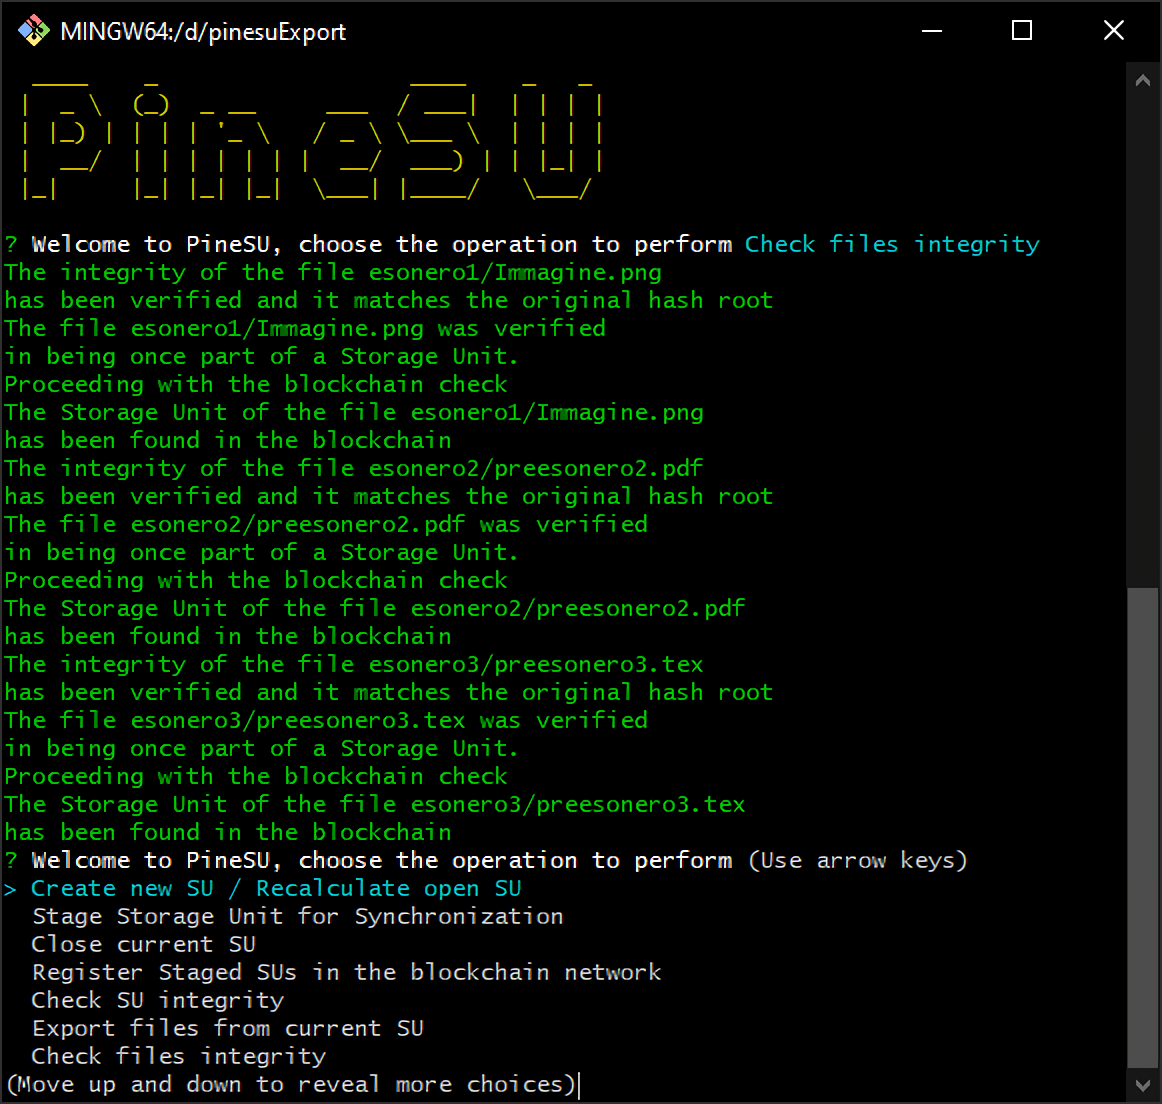
\includegraphics[width=0.9\textwidth]{Figures/verifyFiles}
    \caption{\small{
    L'interfaccia di PineSU durante la verifica dei file esportati da \textsf{secondSample}.
    } % end small
    } % end caption
    \label{fi:vfil}
\end{figure}

Vediamo in Fig.~\ref{fi:vfil} come, per ogni file, viene eseguito un controllo sia locale,
per controllare che non sia stato manomesso, sia remoto, ovvero viene controllato che la SU
di cui lui sostiene di far parte sia stata registrata in blockchain.


\part{Dimostrazioni d'i 'uso per il fine preposto}

Abbiamo potuto osservare come, con il software descritto, si è risolto il problema
della mancanza di una funzione di verifica d’integrità dei file su Git,
andando a sfruttare le tecnologie del Web 3.0 come la Blockchain Ethereum,
sempre con un occhio di riguardo al portafoglio dell’utilizzatore,
servendosi di strutture dati peculiari progettate per permettere un salvataggio economico
e una verifica veloce ed efficiente.

Il progetto ha già subito diverse revisioni e riscritture e si trova ora in uno
stato ben definito e molto fedele alla descrizione fornita
(tralasciando alcuni dettagli poco importanti), tuttavia, nonostante sia un programma
decisamente completo sotto il punto di vista delle funzionalità,
almeno per ciò che avevamo progettato di realizzare, sono presenti alcuni aspetti
su cui si potrebbe ancora lavorare per rendere l’esperienza d’uso molto più adatta
ad affrontare le esigenze lavorative di ogni giorno all’interno di grandi e piccole aziende.

In primis potrebbe essere migliorato il calcolo della Merkle Root corrispondente ad
una singola Storage Unit, infatti per ora la lista di file e directory viene semplicemente
ordinata in ordine alfabetico e da quella viene calcolato un Merkle Tree binario.
Invece, ispirandosi al modo con cui Git traccia le modifiche dei propri file
indentificandoli con il loro hash (come spiegato nella \autoref{sub:git}),
si potrebbe identificare ogni file con l’hash corrispondente e tracciare le modifiche
ogni volta che si effettua un ricalcolo della Storage Unit, evitando quindi di ricalcolare
hash di file che sono rimasti identici, usando possibilmente le funzionalità dei Git commit.

Una seconda aggiunta è sicuramente la creazione del PineSU Smart Contract per la gestione
di registrazioni “forti” su blockchain EVENTUALMENTE POTREI FARLO.

Una terza aggiunta, decisamente più ambiziosa, sarebbe la creazione di una piattaforma
per il salvataggio remoto di Storage Unit, un equivalente a ciò che servizi come GitHub,
BitBucket e GitLab sono per Git.
In questo modo si potrebbe venire incontro anche alle aziende in cui non è
richiesta una grande competenza informatica da parte dei dipendenti
(nonostante l’attuale implementazione di PineSU non si lasci intimidire sotto
il punto di vista dell’essere user-friendly).

\part{Conclusioni e Sviluppi Futuri}

\include{mainmatter/ch7}

\bibliographystyle{plain}
\bibliography{bibliografia}

\cleardoublepage\phantomsection % to fix wrong hyperref to \part{Epilogue}

\end{document}